\documentclass[
letterpaper, % Stock and paper size.
oneside
]{tufte-book}
% packages

\usepackage[utf8]{inputenc}
\usepackage[T1]{fontenc}
\usepackage[english]{babel}
\usepackage[final]{microtype}
\usepackage{hyperref}
\usepackage{enumitem}
\usepackage{csquotes}
\usepackage{framed}
\usepackage{xcolor}
\usepackage{tikz}
\usepackage{forest}
\usepackage{subcaption}
\usepackage{listings}

\usetikzlibrary{shapes.geometric, arrows, positioning}

%\usepackage[lambda,adversary,advantage,asymptotics,sets,landau,probability,operators,primitives]{cryptocode}
\usepackage{amsmath,amssymb,amsthm,mathtools}

\usepackage{capt-of}

% \usepackage{tikz} % Figures
\usepackage{graphicx} % Include figures

% page layout

%\setlrmarginsandblock{0.15\paperwidth}{*}{1} % Left and right margin
%\setulmarginsandblock{0.2\paperwidth}{*}{1}  % Upper and lower margin
%\checkandfixthelayout

% sections

\usepackage[capitalize]{cleveref}
% number down to subsections
\setcounter{secnumdepth}{2}

%\maxsecnumdepth{subsection} % Subsections (and higher) are numbered
%\setsecnumdepth{subsection}
\iffalse
\makeatletter %
\makechapterstyle{standard}{
  \setlength{\beforechapskip}{0\baselineskip}
  \setlength{\midchapskip}{1\baselineskip}
  \setlength{\afterchapskip}{8\baselineskip}
  \renewcommand{\chapterheadstart}{\vspace*{\beforechapskip}}
  \renewcommand{\chapnamefont}{\centering\normalfont\Large}
  \renewcommand{\printchaptername}{\chapnamefont \@chapapp}
  \renewcommand{\chapternamenum}{\space}
  \renewcommand{\chapnumfont}{\normalfont\Large}
  \renewcommand{\printchapternum}{\chapnumfont \thechapter}
  \renewcommand{\afterchapternum}{\par\nobreak\vskip \midchapskip}
  \renewcommand{\printchapternonum}{\vspace*{\midchapskip}\vspace*{5mm}}
  \renewcommand{\chaptitlefont}{\centering\bfseries\LARGE}
  \renewcommand{\printchaptertitle}[1]{\chaptitlefont ##1}
  \renewcommand{\afterchaptertitle}{\par\nobreak\vskip \afterchapskip}
}
\makeatother

\chapterstyle{standard}

\setsecheadstyle{\normalfont\large\bfseries}
\setsubsecheadstyle{\normalfont\normalsize\bfseries}
\setparaheadstyle{\normalfont\normalsize\bfseries}
\setparaindent{0pt}\setafterparaskip{0pt}

% header / footer

\makepagestyle{standard} % Make standard pagestyle

\makeatletter                 % Define standard pagestyle
\makeevenfoot{standard}{}{}{} %
\makeoddfoot{standard}{}{}{}  %
\makeevenhead{standard}{\bfseries\thepage\normalfont\qquad\small\leftmark}{}{}
\makeoddhead{standard}{}{}{\small\rightmark\qquad\bfseries\thepage}
% \makeheadrule{standard}{\textwidth}{\normalrulethickness}
\makeatother                  %

\makeatletter
\makepsmarks{standard}{
\createmark{chapter}{both}{shownumber}{\@chapapp\ }{ \quad }
\createmark{section}{right}{shownumber}{}{ \quad }
\createplainmark{toc}{both}{\contentsname}
\createplainmark{lof}{both}{\listfigurename}
\createplainmark{lot}{both}{\listtablename}
\createplainmark{bib}{both}{\bibname}
\createplainmark{index}{both}{\indexname}
\createplainmark{glossary}{both}{\glossaryname}
}
\makeatother                               %

\makepagestyle{chap} % Make new chapter pagestyle

\makeatletter
\makeevenfoot{chap}{}{\small\bfseries\thepage}{} % Define new chapter pagestyle
\makeoddfoot{chap}{}{\small\bfseries\thepage}{}  %
\makeevenhead{chap}{}{}{}   %
\makeoddhead{chap}{}{}{}    %
% \makeheadrule{chap}{\textwidth}{\normalrulethickness}
\makeatother

\nouppercaseheads
\pagestyle{standard}               % Choosing pagestyle and chapter pagestyle
\aliaspagestyle{chapter}{chap} %

% table of contents

\maxtocdepth{subsection} % Only parts, chapters and sections in the table of contents
\settocdepth{subsection}

\AtEndDocument{\addtocontents{toc}{\par}} % Add a \par to the end of the TOC

% new commands
\fi

\newcommand{\ttt}[1]{\texttt{\detokenize{#1}}}
%\newcommand{\todo}[1]{{{\color{purple} TODO: #1}}}


\renewcommand{\subsubsection}[1]{\paragraph{#1.}}

\newcommand{\concat}{\mathbin{||}}

% TODO: move to correct place
\newcommand{\ppt}{\mathsf{PPT}}
\newcommand{\Sign}{\mathsf{Sign}}
\newcommand{\Ver}{\mathsf{Ver}}
\newcommand{\MAC}{\mathsf{MAC}}
\newcommand{\MACSign}{\mathsf{MAC.Sign}}
\newcommand{\MACVerify}{\mathsf{MAC.Verify}}
\newcommand{\INDCPA}{\text{IND-CPA}}
\newcommand{\xor}{\oplus}
\newcommand{\iv}{\text{IV}}
\newcommand{\AES}{\mathsf{AES}}
\newcommand{\ind}{\cong}

%fields and groups
\newcommand{\id}{\mathsf{id}}
\newcommand{\overflow}{\mathsf{overflow}}
\newcommand{\F}{\mathbb{F}}
\newcommand{\Fp}{\F_p}
\newcommand{\Fq}{\F_q}
\newcommand{\Ftwo}{\F_2}
\newcommand{\Q}{\mathbb{Q}}
\newcommand{\N}{\mathbb{N}}
\newcommand{\Z}{\mathbb{Z}}
\newcommand{\R}{\mathbb{R}}
\newcommand{\C}{\mathbb{C}}
\newcommand{\T}{\mathbb{T}}
\newcommand{\Qbar}{\overline{\Q}}
\newcommand{\G}{\mathbb{G}}
\newcommand{\Vs}{\mathbb{V}}
\newcommand{\Fbar}{\overline{\mathbb{F}}}
\newcommand{\Hash}{\mathsf{Hash}}
\newcommand{\Omtilde}{\widetilde{\Omega}}

\newcommand{\Enc}{\mathsf{Enc}}
\newcommand{\Dec}{\mathsf{Dec}}
\newcommand{\Apply}{\mathsf{Apply}}
\newcommand{\Preproc}{\mathsf{Preproc}}


\DeclareMathOperator*{\E}{\textrm{E}}
\DeclareMathOperator*{\argmax}{arg\,max}
\DeclareMathOperator*{\argmin}{arg\,min}


%vectors, etc.
\newcommand{\av}{\mathbf{a}} \newcommand{\cv}{\mathbf{c}}
\newcommand{\dv}{\mathbf{d}} \newcommand{\ev}{\mathbf{e}}
\newcommand{\rv}{\mathbf{r}} \newcommand{\sv}{\mathbf{s}}
\newcommand{\tv}{\mathbf{t}} \newcommand{\uv}{\mathbf{u}}
%\newcommand{\vv}{\mathbf{v}} \newcommand{\wv}{\mathbf{w}}
\newcommand{\xv}{\mathbf{x}} \newcommand{\yv}{\mathbf{y}}
\newcommand{\zv}{\mathbf{z}} \newcommand{\zerov}{\mathbf{0}}
\renewcommand{\AA}{\mathbf{A}} \newcommand{\BB}{\mathbf{B}}
\newcommand{\CC}{\mathbf{C}} \newcommand{\FF}{\mathbf{F}}
\newcommand{\MM}{\mathbf{M}} \newcommand{\RR}{\mathbf{R}}
\renewcommand{\SS}{\mathbf{S}} \newcommand{\TT}{\mathbf{T}}
\newcommand{\UU}{\mathbf{U}} \newcommand{\XX}{\mathbf{X}}
\newcommand{\YY}{\mathbf{Y}} \newcommand{\KK}{\mathbf{K}}
\newcommand{\A}{\mathcal{A}} \newcommand{\B}{\mathcal{B}}
\newcommand{\dash}{\mbox{---}}
\renewcommand{\O}{\mathcal{O}}
\newcommand{\qq}{\mathfrak{q}}
\newcommand{\QQ}{\mathfrak{Q}}
\newcommand{\ZQ}{\Z_{q}}
\newcommand{\ZZ}{\Z}

\newcommand{\vu}{\mathbf{u}}

\newcommand{\todo}[1]{\noindent {\color{blue} {\footnotesize {\bf TODO}:~{#1}}}}
\newcommand{\hcg}[1]{\todo{HCG: #1}}

\newcommand{\mr}[1]{\ensuremath{\mathrm{{#1}}}}
\newcommand{\la}{\ensuremath{\leftarrow}}
\newcommand{\ra}{\ensuremath{\rightarrow}}
\newcommand{\ala}{\ensuremath{\ \la\ }}
\newcommand{\ara}{\ensuremath{\ \ra\ }}
\newcommand{\rf}{\ensuremath{\overset{\$}{\la}}}

\newcommand{\calA}{\ensuremath{\mathcal{A}}}
\newcommand{\calB}{\ensuremath{\mathcal{B}}}
\newcommand{\calC}{\ensuremath{\mathcal{C}}}
\newcommand{\calD}{\ensuremath{\mathcal{D}}}
\newcommand{\calE}{\ensuremath{\mathcal{E}}}
\newcommand{\calF}{\ensuremath{\mathcal{F}}}
\newcommand{\calG}{\ensuremath{\mathcal{G}}}
\newcommand{\calH}{\ensuremath{\mathcal{H}}}
\newcommand{\calI}{\ensuremath{\mathcal{I}}}
\newcommand{\calJ}{\ensuremath{\mathcal{J}}}
\newcommand{\calK}{\ensuremath{\mathcal{K}}}
\newcommand{\calL}{\ensuremath{\mathcal{L}}}
\newcommand{\calM}{\ensuremath{\mathcal{M}}}
\newcommand{\calN}{\ensuremath{\mathcal{N}}}
\newcommand{\calO}{\ensuremath{\mathcal{O}}}
\newcommand{\calP}{\ensuremath{\mathcal{P}}}
\newcommand{\calQ}{\ensuremath{\mathcal{Q}}}
\newcommand{\calR}{\ensuremath{\mathcal{R}}}
\newcommand{\calS}{\ensuremath{\mathcal{S}}}
\newcommand{\calT}{\ensuremath{\mathcal{T}}}
\newcommand{\calU}{\ensuremath{\mathcal{U}}}
\newcommand{\calV}{\ensuremath{\mathcal{V}}}
\newcommand{\calW}{\ensuremath{\mathcal{W}}}
\newcommand{\calX}{\ensuremath{\mathcal{X}}}
\newcommand{\calY}{\ensuremath{\mathcal{Y}}}
\newcommand{\calZ}{\ensuremath{\mathcal{Z}}}

% -- bold math symbols, for some reason --
\newcommand{\boldalpha}{\ensuremath{\boldsymbol{\alpha}}}
\newcommand{\boldchi}{\ensuremath{\boldsymbol{\chi}}}
\newcommand{\boldtau}{\ensuremath{{\boldsymbol{\tau}}}}
\newcommand{\boldstar}{\ensuremath{\mathbf{*}}}
\newcommand{\bolda}{\ensuremath{\mathbf{a}}}
\newcommand{\boldb}{\ensuremath{\mathbf{b}}}
\newcommand{\boldc}{\ensuremath{\mathbf{c}}}
\newcommand{\boldd}{\ensuremath{\mathbf{d}}}
\newcommand{\bolde}{\ensuremath{\mathbf{e}}}
\newcommand{\boldf}{\ensuremath{\mathbf{f}}}
\newcommand{\boldg}{\ensuremath{\mathbf{g}}}
\newcommand{\boldh}{\ensuremath{\mathbf{h}}}
\newcommand{\boldi}{\ensuremath{\mathbf{i}}}
\newcommand{\boldj}{\ensuremath{\mathbf{j}}}
\newcommand{\boldk}{\ensuremath{\mathbf{k}}}
\newcommand{\boldl}{\ensuremath{\mathbf{l}}}
\newcommand{\boldm}{\ensuremath{\mathbf{m}}}
\newcommand{\boldn}{\ensuremath{\mathbf{n}}}
\newcommand{\boldo}{\ensuremath{\mathbf{o}}}
\newcommand{\boldp}{\ensuremath{\mathbf{p}}}
\newcommand{\boldq}{\ensuremath{\mathbf{q}}}
\newcommand{\boldr}{\ensuremath{\mathbf{r}}}
\newcommand{\bolds}{\ensuremath{\mathbf{s}}}
\newcommand{\boldt}{\ensuremath{\mathbf{t}}}
\newcommand{\boldu}{\ensuremath{\mathbf{u}}}
\newcommand{\boldv}{\ensuremath{\mathbf{v}}}
\newcommand{\boldw}{\ensuremath{\mathbf{w}}}
\newcommand{\boldx}{{\ensuremath{\mathbf{x}}}}
\newcommand{\boldy}{\ensuremath{\mathbf{y}}}
\newcommand{\boldz}{\ensuremath{\mathbf{z}}}
\newcommand{\boldzero}{\ensuremath{\boldsymbol{0}}}
\newcommand{\boldone}{\ensuremath{\boldsymbol{1}}}
\newcommand{\boldpi}{\ensuremath{\boldsymbol{\pi}}}
\newcommand{\boldmu}{\ensuremath{\boldsymbol{\mu}}}
\newcommand{\boldPi}{\ensuremath{\boldsymbol{\Pi}}}

% -- bold italic math symbols, for some reason --
\newcommand{\boldia}{\ensuremath{\boldsymbol{a}}}
\newcommand{\boldib}{\ensuremath{\boldsymbol{b}}}
\newcommand{\boldic}{\ensuremath{\boldsymbol{c}}}
\newcommand{\boldid}{\ensuremath{\boldsymbol{d}}}
\newcommand{\boldie}{\ensuremath{\boldsymbol{e}}}
\newcommand{\boldif}{\ensuremath{\boldsymbol{f}}}
\newcommand{\boldig}{\ensuremath{\boldsymbol{g}}}
\newcommand{\boldih}{\ensuremath{\boldsymbol{h}}}
\newcommand{\boldii}{\ensuremath{\boldsymbol{i}}}
\newcommand{\boldij}{\ensuremath{\boldsymbol{j}}}
\newcommand{\boldik}{\ensuremath{\boldsymbol{k}}}
\newcommand{\boldil}{\ensuremath{\boldsymbol{l}}}
\newcommand{\boldim}{\ensuremath{\boldsymbol{m}}}
\newcommand{\boldin}{\ensuremath{\boldsymbol{n}}}
\newcommand{\boldio}{\ensuremath{\boldsymbol{o}}}
\newcommand{\boldip}{\ensuremath{\boldsymbol{p}}}
\newcommand{\boldiq}{\ensuremath{\boldsymbol{q}}}
\newcommand{\boldir}{\ensuremath{\boldsymbol{r}}}
\newcommand{\boldis}{\ensuremath{\boldsymbol{s}}}
\newcommand{\boldit}{\ensuremath{\boldsymbol{t}}}
\newcommand{\boldiu}{\ensuremath{\boldsymbol{u}}}
\newcommand{\boldiv}{\ensuremath{\boldsymbol{v}}}
\newcommand{\boldiw}{\ensuremath{\boldsymbol{w}}}
\newcommand{\boldix}{\ensuremath{\boldsymbol{x}}}
\newcommand{\boldiy}{\ensuremath{\boldsymbol{y}}}
\newcommand{\boldiz}{\ensuremath{\boldsymbol{z}}}

\newcommand{\transpose}[1]{\ensuremath{{#1}^{\intercal}}}

\newcommand{\boldA}{\ensuremath{\mathbf{A}}}
\newcommand{\boldB}{\ensuremath{\mathbf{B}}}
\newcommand{\boldC}{\ensuremath{\mathbf{C}}}
\newcommand{\boldD}{\ensuremath{\mathbf{D}}}
\newcommand{\boldE}{\ensuremath{\mathbf{E}}}
\newcommand{\boldF}{\ensuremath{\mathbf{F}}}
\newcommand{\boldG}{\ensuremath{\mathbf{G}}}
\newcommand{\boldH}{\ensuremath{\mathbf{H}}}
\newcommand{\boldI}{\ensuremath{\mathbf{I}}}
\newcommand{\boldJ}{\ensuremath{\mathbf{J}}}
\newcommand{\boldK}{\ensuremath{\mathbf{K}}}
\newcommand{\boldL}{\ensuremath{\mathbf{L}}}
\newcommand{\boldM}{\ensuremath{\mathbf{M}}}
\newcommand{\boldN}{\ensuremath{\mathbf{N}}}
\newcommand{\boldO}{\ensuremath{\mathbf{O}}}
\newcommand{\boldP}{\ensuremath{\mathbf{P}}}
\newcommand{\boldQ}{\ensuremath{\mathbf{Q}}}
\newcommand{\boldR}{\ensuremath{\mathbf{R}}}
\newcommand{\boldS}{\ensuremath{\mathbf{S}}}
\newcommand{\boldT}{\ensuremath{\mathbf{T}}}
\newcommand{\boldU}{\ensuremath{\mathbf{U}}}
\newcommand{\boldV}{\ensuremath{\mathbf{V}}}
\newcommand{\boldW}{\ensuremath{\mathbf{W}}}
\newcommand{\boldX}{\ensuremath{\mathbf{X}}}
\newcommand{\boldY}{\ensuremath{\mathbf{Y}}}
\newcommand{\boldZ}{\ensuremath{\mathbf{Z}}}

\newcommand{\deq}{\mathrel{\mathop:}=}
\newcommand{\zo}{\ensuremath{\{0,1\}}} % bits
\newcommand{\bin}{\zo}
\newcommand{\zon}{\ensuremath{\{0,1\}^n}} % bits

% Theorem definitions

\theoremstyle{plain}
%\newtheorem{theorem}{Theorem}[section]
\newtheorem{theorem}{Theorem}[section]
\newtheorem{inf-theorem}{Informal Theorem}[section]
\newtheorem*{rtheorem}{Theorem}
\newtheorem{lemma}[theorem]{Lemma}
\newtheorem{corollary}[theorem]{Corollary}
\newtheorem*{claim}{Claim}
\theoremstyle{remark}
\newtheorem{remark}[theorem]{Remark}
\theoremstyle{definition}
\newtheorem*{theorems}{Theorem}
\newtheorem{defn}[theorem]{Definition}
\newtheorem{definition}[theorem]{Definition}
\newtheorem{fact}[theorem]{Fact}
\newtheorem{conjecture}[theorem]{Conjecture}
\newtheorem{const}[theorem]{Construction}
\newtheorem{attackgame}[theorem]{Attack Game}


\newtheoremstyle{goal}% name of the style to be used
  {\topsep}% measure of space to leave above the theorem. E.g.: 3pt
  {\topsep}% measure of space to leave below the theorem. E.g.: 3pt
  {\normalfont}% name of font to use in the body of the theorem
  {0pt}% measure of space to indent
  {\bfseries}% name of head font
  {: } %punctuation between head and body
  { }% space after theorem head; " " = normal interword space
  {\thmname{#1}\thmnumber{ #2}\thmnote{ (#3)}}
\theoremstyle{goal}
\newtheorem{sgoal}{Security Goal}
\newtheorem{fgoal}{Functionality Goal}

\newtheoremstyle{pstyle}% name of the style to be used
  {2pt}% measure of space to leave above the theorem. E.g.: 3pt
  {2pt}% measure of space to leave below the theorem. E.g.: 3pt
  {\itshape}% name of font to use in the body of the theorem
  {0pt}% measure of space to indent
  {\itshape}% name of head font
  {: } %punctuation between head and body
  { }% space after theorem head; " " = normal interword space
  {\thmname{#1}\thmnumber{ #2}\thmnote{ (#3)}}
\theoremstyle{pstyle}
\newtheorem{prop}[theorem]{Proposition}
%% custom macros

\newcommand{\esm}[1]{\ensuremath{#1}}
\newcommand{\ms}[1]{\esm{\mathsf{#1}}}

\newcommand{\prg}{\ms{PRG}}
\newcommand{\prf}{\ms{PRF}}
\newcommand{\prp}{\ms{PRP}}

\newcommand{\poly}{\operatorname{poly}}
\newcommand{\polylog}{\operatorname{polylog}}
\newcommand{\negl}{\operatorname{negl}}

\newcommand{\ord}[1]{\esm{{#1}^{\mr{th}}}}

\newcommand{\hyb}{\ms{Hyb}}
\newcommand{\Funs}{\ms{Funs}}
\newcommand{\getsr}{\rgets}
\newcommand{\rgets}{\mathrel{\mathpalette\rgetscmd\relax}}
\newcommand{\rgetscmd}{\ooalign{$\leftarrow$\cr
    \hidewidth\raisebox{1.2\height}{\scalebox{0.5}{\ \rm R}}\hidewidth\cr}}

%\getsr with proper vertical space.    
% this makes it typeset better in subscripts
\def\getsrx{\mathrel{%
    \mathchoice{\GETSRX}{\GETSRX}{\scriptsize\GETSRX}{\tiny\GETSRX}%
}}
\def\GETSRX{{%
\setbox0\hbox{$\gets$}%
\rlap{\hbox to \wd0{\hss$\raisebox{1.2\height}{\scalebox{0.5}{\ R}}$\hss}}\box0
}}

\newcommand{\Unif}{\ms{Unif}}

\newcommand{\iseq}{\stackrel{?}{=}}

\newcommand{\appc}{\stackrel{c}{\approx}}
\newcommand{\apps}{\stackrel{s}{\approx}}
\newcommand{\abs}[1]{\left| #1 \right|}

\newcommand{\classP}{\ms{P}}
\newcommand{\classBPP}{\ms{BPP}}
\newcommand{\classNP}{\ms{NP}}
\newcommand{\Ppoly}{\ms{P}/\ms{poly}}
\newcommand{\NCone}{\ms{NC^1}}

\newcommand{\round}[1]{\left\lfloor #1 \right\rceil}
\newcommand{\floor}[1]{\left\lfloor #1 \right\rfloor}
\newcommand{\ceil}[1]{\left\lceil #1 \right\rceil}
\newcommand{\iprod}[1]{\left\langle #1 \right\rangle}
\newcommand{\norm}[1]{\left\| #1 \right\|}
\newcommand{\set}[1]{\left\{ #1 \right\}}

\newcommand{\Zp}{\Z_p}
\newcommand{\Zq}{\Z_q}

\newcommand{\subind}[2]{{#1}^{(#2)}}

\newcommand{\eqq}{\stackrel{?}{=}}

\newcommand{\Otilde}{\widetilde{O}}
\newcommand{\Otildel}{\widetilde{O}_\lambda}
\newcommand{\Omtildel}{\widetilde{\Omega}_\lambda}

\newcommand{\hc}{\ms{hc}}

\newcommand{\xstar}{x^*}
\newcommand{\ystar}{y^*}

\newcommand{\DDHAdv}{\ms{DDHAdv}}
\newcommand{\PRFAdv}{\ms{PRFAdv}}
\newcommand{\PRGAdv}{\ms{PRGAdv}}

\newcommand{\ct}{\ms{ct}}

\newcommand{\View}{\ms{View}}
%\newcommand{\view}{\ms{View}_{\calV^*}}
\newcommand{\Sim}{\ms{Sim}}


\newcommand{\bv}{\mathbf{b}}
\newcommand{\Bm}{\mathbf{B}}
\newcommand{\Rm}{\mathbf{R}}
\newcommand{\Gm}{\mathbf{G}}

\newcommand{\pro}[1]{\langle #1 \rangle}
\newcommand{\Comm}{\ms{Commit}}
\newcommand{\cSAT}{\ms{circuit}\text{-}\ms{SAT}}

\newcommand{\op}{\ms{op}}
\newcommand{\ck}{\ms{ck}}
\newcommand{\st}{\ms{st}}
\newcommand{\shint}{\hint_s}
\newcommand{\chint}{\hint_c}
\newcommand{\rhint}{\hint_r}
\newcommand{\fhint}{\hint_f}
\newcommand{\row}{\ms{row}}
\newcommand{\col}{\ms{col}}

\newcommand{\sig}{\sigma}

\newcommand{\sk}{{\ms{sk}}}
\newcommand{\pk}{\ms{pk}}
\newcommand{\pp}{\ms{pp}}
\newcommand{\vk}{\ms{vk}}


\newcommand{\seed}{\ms{seed}}
\newcommand{\db}{\ms{db}}
\newcommand{\qu}{\ms{qu}}
\newcommand{\irow}{i_{\text{row}}}
\newcommand{\icol}{i_{\text{col}}}
\newcommand{\adv}{\ms{adv}}
\newcommand{\off}{\ms{off}}

\newcommand{\hreq}{q_h}
\newcommand{\hint}{\mathsf{hint}}

\newcommand{\ans}{\mathsf{ans}}
\newcommand{\Query}{\mathsf{Query}}
\newcommand{\Decide}{\mathsf{Decide}}
\newcommand{\Setup}{\mathsf{Setup}}
\newcommand{\Hint}{\mathsf{Hint}}
\newcommand{\SAns}{\mathsf{Answer}}
\newcommand{\Ans}{\SAns}
\newcommand{\Answer}{\SAns}

\newcommand{\defeq}{\coloneqq}
\newcommand{\distadv}{\mathsf{DistAdv}}
\newcommand{\piradv}{\mathsf{PIRadv}}
\newcommand{\epspir}{\epsilon_\mathsf{pir}}
\newcommand{\epsbox}{\epsilon_\mathsf{box}}
\newcommand{\Supp}{\mathsf{Supp}}
\newcommand{\Bern}{\mathsf{Bernoulli}}


\newcommand{\PS}{\Psi}
\mathchardef\mhyphen="2D % Define a "math hyphen"
\newcommand{\pPRF}{\mathsf{pPRF}}
\newcommand{\psk}{\sk_\mathsf{p}}
\newcommand{\pS}{S_\mathsf{p}}
\newcommand{\pb}{b_\mathsf{p}}
\newcommand{\Kp}{{\mathcal{K}_{\mathsf{p}}}}
\newcommand{\noti}{{\bar{i}}}


\newcommand{\Gen}{\mathsf{Gen}}
\newcommand{\Punc}{\mathsf{Punc}}
\newcommand{\Eval}{\mathsf{Eval}}
\newcommand{\InSet}{\mathsf{InSet}}
\newcommand{\Choose}{\mathsf{Choose}}
\newcommand{\GenWith}{\mathsf{GenWith}}
\newcommand{\Shift}{\mathsf{Shift}}
\newcommand{\Derive}{\mathsf{Derive}}

\newcommand{\PRFGen}{\mathsf{PRFGen}}
\newcommand{\PRFPunc}{\mathsf{PRFPunc}}
\newcommand{\PRFEval}{\mathsf{PRFEval}}

\newcommand{\PSadv}{\mathsf{PSAdv}}
\newcommand{\PSseladv}{\PS\mathsf{selAdv}}
\newcommand{\pPRFadv}{\mathsf{pPRFAdv}}
\newcommand{\pPRFadvu}{{\mathsf{pPRFAdv}^\mathrm{unp}}}
\newcommand{\prstuple}{(\Gen,\Punc,\Eval)}
\newcommand{\PStuple}{(\Gen,\allowbreak\Punc,\allowbreak\Eval)}
\newcommand{\PRFtuple}{(\PRFGen,\allowbreak\PRFPunc,\allowbreak\PRFEval)}
\newcommand{\Pituple}{\Pi =\allowbreak (\Setup,\allowbreak\Hint,\allowbreak\Query,\allowbreak\SAns,\allowbreak\CRecon)}
\newcommand{\PreTuple}{\PiPre =\allowbreak (\Setup,\allowbreak\Query,\allowbreak\Hint,\allowbreak\Ans,\allowbreak\Recon)}

\newcommand{\getsrtiny}{\mathrel{\mathpalette{
    \ooalign{\text{\tiny{$\leftarrow$}}\cr%
    \hidewidth\raisebox{1\height}{\scalebox{0.7}{\,\rm{\tiny R}}}\hidewidth\cr}
}\relax}}

\newcommand{\PrTiny}[1]{\Pr_{\scriptscriptstyle{#1}}} 

\newcommand{\ia}{{i_{\mathsf{adv}}}}
\newcommand{\ip}{i_{\mathsf{punc}}}
\newcommand{\ig}{i_{\mathsf{guess}}}
\newcommand{\ipir}{i_{\mathsf{pir}}}
\newcommand{\dummy}{\mathsf{{dummy}}}
\newcommand{\new}{\mathsf{{new}}}
\newcommand{\sknew}{\sk_{\ms{new}}}
\newcommand{\skright}{\sk_{\ms{right}}}
\newcommand{\skleft}{\sk_{\ms{left}}}
\newcommand{\Prbig}[1]{\Pr\Big[ #1 \Big]}

\newcommand{\ol}{1^{\lambda}}
\newcommand{\fk}{\ms{k}}
\newcommand{\fkp}{\ms{k}_{\ms{p}}}


\makeatletter
\def\moverlay{\mathpalette\mov@rlay}
\def\mov@rlay#1#2{\leavevmode\vtop{%
   \baselineskip\z@skip \lineskiplimit-\maxdimen
   \ialign{\hfil$\m@th#1##$\hfil\cr#2\crcr}}}
\newcommand{\charfusion}[3][\mathord]{
    #1{\ifx#1\mathop\vphantom{#2}\fi
        \mathpalette\mov@rlay{#2\cr#3}
      }
    \ifx#1\mathop\expandafter\displaylimits\fi}
\makeatother

% Vectors and Matrices
\renewcommand{\vec}[1]{\mathbf{#1}}
\newcommand{\mat}[1]{\ensuremath{\mathbf{#1}}\xspace} % Matrix

\newcommand{\Accept}{\ensuremath{\mathsf{Accept}}\xspace} 
% Algorithms
\newcommand{\GenToken}{\ensuremath{\mathsf{GenToken}}\xspace}
\newcommand{\KDer}{\ensuremath{\mathsf{KDer}}\xspace} % Key Derivation
\newcommand{\KeyComp}{\ensuremath{\mathsf{KeyComp}}\xspace} % Key Compression
\newcommand{\NextStep}{\ensuremath{\mathsf{NextStep}}\xspace}
\newcommand{\OAccess}{\ensuremath{\mathsf{OAccess}}\xspace} % Oblivious Access
\newcommand{\PoK}[2]{\ensuremath{\mathsf{PoK}\left\{#1 : #2\right\}}\xspace}
\newcommand{\ReRand}{\ensuremath{\mathsf{ReRand}}\xspace} % Re-randomize
\newcommand{\Read}{\ensuremath{\mathsf{Read}}\xspace}
\newcommand{\Write}{\ensuremath{\mathsf{Write}}\xspace}
\newcommand{\access}{\ensuremath{\mathsf{Access}}\xspace} % Access
\newcommand{\aggregate}{\ensuremath{\mathsf{Agg}}\xspace} % Aggregate
\newcommand{\auth}{\ensuremath{\mathsf{Auth}}\xspace}
\newcommand{\com}{\ensuremath{\mathsf{Com}}\xspace}
\newcommand{\constrain}{\ensuremath{\mathsf{Constrain}}\xspace} % Constrain
\newcommand{\corr}{\ensuremath{\mathsf{Corr}}\xspace}
\newcommand{\delegate}{\ensuremath{\mathsf{Del}}\xspace}
\newcommand{\enroll}{\ensuremath{\mathtt{enrl}}\xspace}
\newcommand{\evict}{\ensuremath{\mathsf{Evict}}\xspace} % Evict
\newcommand{\fetch}{\ensuremath{\mathsf{Fetch}}\xspace} % Fetch
\newcommand{\finalize}{\ensuremath{\mathsf{Finalize}}\xspace}
\newcommand{\foward}{\ensuremath{\mathsf{Fwd}}\xspace}
\newcommand{\gen}{\ensuremath{\mathsf{Gen}}\xspace}
\newcommand{\join}{\ensuremath{\mathsf{Join}}\xspace}
\newcommand{\judge}{\ensuremath{\mathsf{Judge}}\xspace} % Judge
\newcommand{\link}{\ensuremath{\mathsf{Link}}\xspace}
\newcommand{\open}{\ensuremath{\mathsf{Open}}\xspace}
\newcommand{\prove}{\ensuremath{\mathsf{Prove}}\xspace}
\newcommand{\rand}{\ensuremath{\mathsf{Rand}}\xspace}
\newcommand{\register}{\ensuremath{\mathsf{Reg}}\xspace}
\newcommand{\request}{\ensuremath{\mathsf{Request}}\xspace}
\newcommand{\preprocess}{\ensuremath{\mathsf{Preprocess}}\xspace}
\newcommand{\respond}{\ensuremath{\mathsf{Respond}}\xspace}
\newcommand{\rotate}{\ensuremath{\mathsf{Rotate}}\xspace}
\newcommand{\setup}{\ensuremath{\mathsf{Setup}}\xspace}
\newcommand{\encrypt}{\ensuremath{\mathsf{Encrypt}}\xspace}
\newcommand{\decide}{\ensuremath{\mathsf{Decide}}\xspace}
\newcommand{\store}{\ensuremath{\mathsf{store}}\xspace}
\newcommand{\test}{\ensuremath{\mathsf{Test}}\xspace}
\newcommand{\trace}{\ensuremath{\mathsf{Trace}}\xspace}
\newcommand{\update}{\ensuremath{\mathsf{Update}}\xspace}
\newcommand{\validate}{\ensuremath{\mathtt{val}}\xspace}
\newcommand{\query}{\ensuremath{\mathsf{Query}}\xspace}
\newcommand{\answer}{\ensuremath{\mathsf{Answer}}\xspace}
\newcommand{\Index}{\ensuremath{\mathsf{Index}}\xspace}

\newcommand{\Conv}{\mathsf{Conv}}
\newcommand{\Share}{\mathsf{Share}}
\newcommand{\recover}{\mathsf{Recover}}
\newcommand{\Decode}{\mathsf{Dec}}
\newcommand{\expand}{\mathsf{Decomp}}
\newcommand{\expandinv}{\mathsf{Recomp}}
\newcommand{\Combine}{\mathsf{Combine}}
\newcommand{\Findcover}{\mathsf{FindCover}}
\newcommand{\Tofuncs}{\mathsf{ToFuncs}}

\newcommand{\tofunc}{\mathsf{Expand}}
\newcommand{\Bad}{\mathsf{Bad}}
\newcommand{\cross}{\times}



\lstset{basicstyle=\ttfamily,breaklines=true}


\author{6.1600 Staff}
\title{6.1600\\Foundations of\\Computer Security}

\usepackage{lipsum} % Just to put in some text

\begin{document}

\mainmatter

\maketitle

%\begin{abstract}
%	This is an introduction to the class
%\end{abstract}
\clearpage

\tableofcontents*
\clearpage

%\mainmatter

\chapter{What is Security?}

\chapter{What is Security?}

\section{Overview}

The goal of this course is to give you an overview of the 
most important ``Big Ideas'' on securing computer systems.
Throughout the course, we will touch on ideas from the fields
of computer security, cryptography, and (to some extent)
computer systems.

\iffalse
\textbf{Big Idea}: Big ideas for securing computers.
\begin{itemize}
	\item Lectures: ask questions!
	\item Labs (coding) + psets (theory)
	\item Midterm + final
\end{itemize}
\fi

\section{What is Security?}
Security is a very broad property, but generally
the goal of computer security 
is to ensure that a particular computer system is 
``behaves correctly'' even in the
face of an ``adversary'' (or ``attacker'') whose goal is to foil the
system.
\marginnote{We will use the terms ``adversary'' and ``attacker''
interchangeably throughout this course.}

To achieve this goal, we will need some kind of
systematic plan.
That is, we will have to carefully define 
what it means for our system to ``behave correctly''
and we will have to specify the class of 
``adversaries'' against which we want to defend.

For the purposes of this course, we will typically
structure our plan in terms of three components:
a \emph{goal}, 
a \emph{threat model}, and
an \emph{implementation}.

\begin{itemize}
  \item \textbf{Goal:} 
    The security goal defines what we want our system to achieve.
    For example, a informal goal might be that ``only Alice can read the file $F$,''
    or ``if anyone tampers with the file $F$, Alice will detect it.''
    As you will learn throughout the course, figuring out exactly what your
    security goal should be is often quite subtle and challenging.

  \item \textbf{Threat model:} 
    The threat model (or ``adversary model'') specifies the class of 
    adversaries against which we want to defend.
    Or, put another way, the threat model specifies the adversary's power:
    what can the adversary do in trying to break our security goal?
    By defining a threat model, we can make it
    tractable to achieve a security goal. 
    For example, in analyzing the security of a password-based login system,
    our threat model might specify that 
    the adversary can guess passwords, but cannot steal the server.
  \item \textbf{Implementation:}
    The implementation is how we achieve the goal.
    For example, we might set permissions on a file $F$, 
    use Linux to enforce those permissions, 
    and require two-factor authentication to access the system.
\end{itemize}

Together, the goal and the threat model create our
\textit{definition} of security.\marginnote{When you read
about security failures in the news, it is worth trying
to understand whether the failure arose from a problem with the
goal, the threat model, or the implementation.}
As such, they
cannot be ``wrong''---the goal might turn out to
not be exactly what we needed, 
the threat model might not have captured all of
the attacks that our system might actually face
in the real world, and the system designer might
be surprised when they discover this,
but together the goal and threat model define 
the security properties that we set out to achieve.
The implementation, on the other hand, can definitely be wrong---if 
the implementation does not guarantee the goal under the threat model, due to bugs or oversights or supply chain vulnerabilities or anything else, the implementation has a mistake.

\subsection{Security is Hard}

Building secure systems is challenging.
There are at least two broad reasons for this.

\paragraph{Secure systems must defend against worst-case behavior.}
First, a secure system must defend against
\emph{all possible attacks} within the scope of 
the threat model.
In contrast, when we are just concerned about functionality or
correctness, we are often satisfied with a system 
that performs well for the cases that users care about.
\marginnote{Some developers do worry about correctness
of their system for all possible inputs and corner cases; this is
is indeed the mindset that is often necessary for security.}
In other words, security is concerned with behavior in
\emph{worst-case situations}, while correctness is often
about behavior in \emph{expected situations}.

For example, suppose that we have
a student-information system that should achieve the security
goal: ``\textbf{only} TAs can access grades.''
It is easy to test if a random sample of TAs can
access grades (correctness), but it is much harder to test whether
there is some sequence of interactions that allow
\textit{anyone else} to access the grades (security).

\paragraph{An implementation can never defend against all possible threats.}
When we specify a threat model, we delimit the set of adversaries 
against which our implementation must defend.
But real-world adversaries can behave in ways that are 
outside of our threat model and thereby violate our security goals.

For example, someone besides a TA might be able to
access the grades by:
\begin{itemize}
	\item finding a bug in the server software,
	\item breaking into a TA's office,
        \item compromise the TA's laptop,
	\item stealing the password to an administrator's account,
	\item tricking a TA into disclosing grades,
	\item breaking the server's cryptography,
	\item getting a job at the registrar and making herself a TA.
\end{itemize}

And the list never ends. Because our threat model cannot capture all
possible threats, \textbf{security is never perfect}.
There will essentially always be \textit{some} attacker than can break your system.

This is why we need a threat model: the threat
model defines what kinds of attacks we worry about
and which we decide are out of scope.

\subsection{Designing security goals and a threat model}
Specifying security goals and
a threat model is all about comparing
the cost of defending against an attack with the
cost of that attack if it were to happen.
It is almost always impractical to exactly calculate
these costs, but this framework is useful
conceptually.
Cheap defenses that block major
holes are likely to be worth implementing, but
defending against an esoteric RF side channel that
could leak unimportant information is likely not.

Building a threat model always requires iterating---you will not get it right on the first try.
There is likely to be some type of attack that you didn't consider at first that ends up being important.

\subsection{Designing an implementation}
We will focus largely in this class on techniques
that have a big payoff---methods of developing
software and tools to use that eliminate entire
classes of attacks (or make them much harder). 

\section{Examples}

We give a handful of examples of security failures arising from poor
choices of security goals or threat model.

\subsection{Bad Goals}
\subsubsection{Business-class airfare}
An airline tried to add value to their
business-class tickets by allowing ticket-holders to 
change the ticket (i.e., the departure date, origin, and destination)
at any time with no fee.
One customer realized that they could board the flight
\textit{then} change their ticket.
The customer could then take an unlimited number of
business-class flights for the price of one.

In this case, the airline's goal did not meet
their real needs---perhaps they needed to add
an additional goal of the form ``every time someone takes a flight,
we get paid.''

\subsubsection{Sarah Palin's Email}
Sarah Palin had a Yahoo email account, and Yahoo
used security questions for password reset---their
goal may have been something like ``no one can
reset a user's password unless they know all of
the answers to the user's security questions.''
(The security questions are typically things like
``What is your mother's maiden name?'')
As it turned out, it was possible to find the answer
to all of Palin's account-recovery security questions 
on the Internet.\autocite{palin}
Yahoo's implementation may have been perfect, but their
goal did not provide any meaningful security for certain users.

\subsubsection{Instruction Set Architecture (ISA) Specification}
When defining ISAs for processors, designers did
not think that timing was important, and
processors could take a variable number of cycles
to execute a particular instruction.
This had big benefits for performance and for
compatibility, but as we'll talk about later in
the semester, researchers have recently exploited
this timing variability to perform sophisticated
attacks on wide ranges of processors.\autocite{hill:spectre-meltdown}
The processor implementation matched the
specification, but the specification itself
allowed for this attack.

\subsubsection{Complicated access-control policies}
A school in Fairfax, Virginia used an online
course-management software with a somewhat complex
access-control structure: each teacher is in charge of some
class, each class has many students, and each
student has many files. Teachers cannot access
student's files, and there is also
a superintendent that has access to all the files.
Teachers are able to change their students'
passwords, and are able to add students to their
class. It turned out that a teacher could add the
superintendent as a student, change the
superintendent's password, and then access all
files via the superintendent's account.
While each of the access-control policies individually
sounds reasonable, together they lead to a bad outcome.


\subsubsection{Mat Honan's Gmail Account}
A journalist for wired named Mat Honan had his Gmail account compromised via a clever attack.\autocite{honan}
Honan had a Gmail account.
Gmail's reset-password feature avoided using security questions, and instead used a backup email account.
The attacker triggered the reset-password feature, which sent a reset link
to Honan's Apple email account.

The attacker then attempted to gain access to Honan's Apple email account.
The attacker triggered the reset-password feature on the Apple account.
Apple's reset-password feature, in turn, required Honan's address and the last four digits of the credit card number.
The attacker was able to find Honan's address publicly, but could not easily find his credit-card number.

The attacker found this credit-card information through Honan's Amazon account.
Amazon, which knew his credit card number, required a full credit-card in order to reset an account.
However, Amazon allowed buying something for a certain account without logging in, 
so long as you provide a new credit card number.
It also allowed \textit{saving} this new credit card number to the user's Amazon account.
So, the attacker made a purchase on Amazon with the attacker's credit card.
Then, the attacker saved their own credit card number to Honan's Amazon account.
Next, the attacker triggered Amazon's reset-password feature, and---using the credit-card
number saved to the account---were able to reset Honan's 
Amazon password and access his Amazon account.
The attacker was then able to see the last four
digits of Honan's real credit card within his
Amazon account, use that to reset his Apple mail
account, and then use that to reset Honan's Gmail
account.

Complex chains of systems like this can be very hard to reason about,
but these interactions ultimately are security-critical.

\subsection{Bad Threat Models}

\subsubsection{Assuming specific strategy: CAPTCHA}
CAPTCHAs were designed to be expensive to
solve via automation, but easy for a human to read.
Indeed it might be expensive to build an optical-character recognition 
system for CAPTCHAs in general, but attackers who want
to bypass CAPTCHAs do not do this.
Instead, they set up computer centers in countries where the cost of
labor is cheap. Attackers then pay people working in these 
centers to solve CAPTCHAs.\autocite{motoyama:recaptchas}
The result is that it costs some fraction of
a cent to solve a CAPTCHA. 
The cost of solving a CAPTCHA is still non-zero,
but the cost is much lower than the system designers
may have intended.

\subsubsection{Computational Power: DES}
There used to be an encryption standard called DES that had $2^{56}$ possible keys.
At the time that it was designed, the U.S.~government standards agencies asserted that it was
secure against even powerful attackers,
but today a modern computer can try all $2^{56}$ keys at only modest cost.\marginnote{For
example, \url{https://crack.sh/} uses an array of FPGAs to provide a service that
exhaustively checks all possible keys.}
(Academic researchers even at the time of DES's
design understood that 56-bit keys were not large
enough to prevent exhaustive
cryptanalysis.\autocite{DH77})

Because of the weakness of DES against modern computers,
everyone using the standard had to upgrade their block ciphers.
For example, MIT had to switch from using DES for authentication 
to newer block ciphers with longer keys, such as AES.

\subsubsection{Dependencies: Two-factor authentication (2FA) via SMS}
Many 2FA systems use a text message for authentication, but an attacker then
just needs to convince the clerk at the AT\&T store to give them a new SIM card for your phone number.
\marginnote{These attacks are often called ``SIM swapping'' or ``SIM hijacking''.}

\subsubsection{Software Versions: Xcode}\label{sec:intro:xcode}
iPhone apps are normally created and compiled on a developer's machine, sent to Apple's App Store, and sent to iPhones from there. iPhone apps are created using a tool called Xcode that is normally downloaded from Apple servers. However, Xcode is a big piece of software and for developers behind China's firewall, it was very slow to download. Someone within China set up a much faster mirror of Xcode, and lots of developers in China used the version of Xcode from this mirror. However, this mirror was not serving exactly Apple's version of Xcode---instead, it was serving a slightly modified version of Xcode that would inject some malicious code into every app that was compiled with it. This took a long time to detect.
\marginnote{The Wikipedia article on XcodeGhost, \url{https://en.wikipedia.org/wiki/XcodeGhost}, provides more details about this attack.}

\subsection{Problematic Implementations}
Bugs, misconfigurations, and other mistakes are the most common cause of security issues. A rule of thumb to keep in mind is that every 1000 lines of code will have around 1 bug. This is a very rough estimate, but the basic idea is that more code will have more bugs. An effective strategy to reduce security vulnerabilities is to reduce the amount of code in your system.

\subsubsection{Missing Checks: iCloud}
Apple's iCloud performs many functions---email, calendar, storage, and Find my iPhone. Each of these had their own way of logging in, but across all of them a common goal was to limit the attacker's ability to guess a user's password. To do this, they added rate limiting to all the login interfaces, allowing something like only 10 login attempts per hour---but they forgot the Find my iPhone login interface.\autocite{icloud} Because this authentication code was duplicated all over the place, there were many places to remember to add this rate limiting, but the attacker only needed one weak login interface to brute-force a password. In general, avoiding this repition will make it much easier to build a secure system.

\subsubsection{Insecure Defaults}
When you set up a new service, they almost always come with some defaults to make the setup simpler. Wi-Fi routers come with default passwords, AWS S3 buckets come with default permissions, and so on. These defaults can be convenient, but they are very important to security because many people will forget or neglect to change the default. Because of this, the default becomes the way that the system operates. In order to build a secure system, it is important that the default is secure.

\section{What are the general principles for secure system design?}
\subsection{Goals and Threat Models}
\begin{itemize}
	\item Create simple, general goals.
	\item Avoid assumptions (such as ``no one else will be able to get a user's SIM card'') through better designs.
	\item Learn and iterate.
	\item Practice Defense in Depth: don't rely on one single defense for all your security---it is useful to use backup defenses to guard against bugs that will inevitably come up in one defense.
\end{itemize}

\subsection{Implementation}
\begin{itemize}
	\item A simpler system will lead to fewer problems.
	\item Factor out the security-critical part into a small separate system or piece of code (for example, hardware security keys).
	\item Reuse well-designed code, such as well-tested crypto libraries.
	\item Understand and test the corner cases.
\end{itemize}





\part{Authentication}
\chapter{Authenticating People}

\chapter{Authenticating People}


\section{Authentication}
In this class, we will talk a lot about requests
going to a computer system.
And a lot of security comes down to looking at that request and deciding
how to handle it.
For this, it is crucial to know
\textit{who} issued the request. Then, we can
decide whether the class should be allowed.

Typically, a computer system performs two steps before processing
a request:
\begin{enumerate}
  \item \textbf{Authenticate:} Identify the person or machine (the ``\emph{principal}'') making the request.
  \item \textbf{Authorize:} Decide if the principal is authorized to make the request.
\end{enumerate}

\section{Passwords}
Passwords are the most widespread method 
that humans use to authenticate to computer systems.
We use passwords to authenticate to ATMs,
our phones, our computers, and so on.

Examples of human-chosen passwords are:
\begin{itemize}
	\item \ttt{password}
	\item \ttt{PaSsW0rd1!}
	\item \ttt{purple-student-hat}
\end{itemize}

Which of these passwords are ``good'' and which
are ``bad?''
Many sites would let you use
\ttt{PaSsW0rd1!} as your password but would not allow
you to use \ttt{purple-student-hat}.
However, what really matters is the adversary's
uncertainty about your password.
That is, what we really care about is that the adversary
will not be able to guess your password in
a small number of guesses.

%And most likely, they will guess the
%most common passwords first.

\begin{figure}
  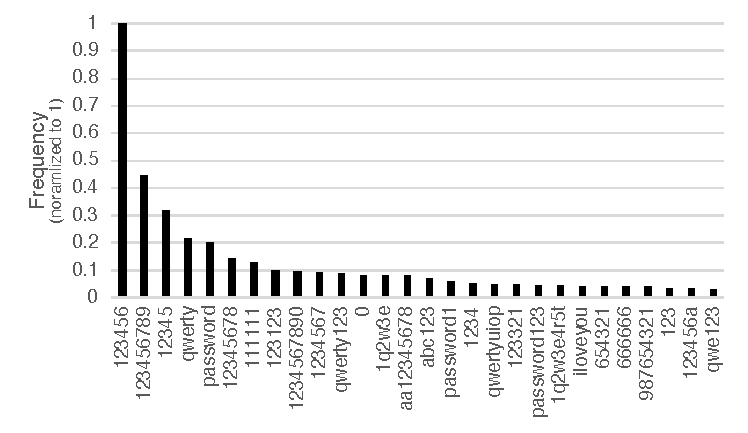
\includegraphics[width=\textwidth]{figs/password-dist.pdf}
  \caption{The most common passwords, according to
  NordPass (\url{https://nordpass.com/most-common-passwords-list/}),
  sorted by their frequency descending.
  A small number of common passwords dominate.
  \todo{Fix the $y$-axis here.}}
\end{figure}

Ideally, we would want all passwords to be equally as likely,
from the adversary's perspective.
But that is not the case.
People have to remember their passwords,
and it turns out that many people are likely to choose the same password.

\marginnote[-2in]{
  \begin{tabular}{cc}
    Rank & Password \\
1 & \ttt{123456}\\
2 & \ttt{123456789}\\
    3 & 12345\\
    4 & qwerty\\
    5& password\\
    6& 12345678\\
    7& 111111\\
    8& 123123\\
    9& 1234567890\\
    10& 1234567\\
    11& qwerty123\\
    12& 000000\\
    13& 1q2w3e\\
    14& aa12345678\\
    15& abc123\\
    16& password1\\
    17& 1234\\
    18& qwertyuiop\\
    19& 123321\\
    20& password123
  \end{tabular}
  \medskip
  \captionof{table}{The most popular passwords in 2021, according to 
  NordPass, \url{https://nordpass.com/most-common-passwords-list/}.}
}

How do we convince humans to choose hard-to-guess passwords? 

\begin{itemize}
  \item \emph{Require longer passwords?} If someone tries to use 
    \ttt{abc123} as a password but it's not long
    enough, they might use \ttt{abc123456}---but
    this doesn't really add much uncertainty.
    There are standard ways to lengthen passwords,
    and a clever attacker will try these first.
  \item \emph{Prohibit using common English words in passwords?}
    It's not clear that this is a good idea.
    Five randomly chosen words from the dictionary will
    form a strong password, and prohibiting English words
    in passwords may make passwords much more difficult to remember.
      
  \item \emph{Force password changes?}
    This makes it harder for users to remember their password, and
    may actually cause users to choose easier-to-guess passwords
    (since these may be easier to remember).
    Forcing a password change may be more effective if the system has
    suffered a breach and the users' passwords have leaked out.

  \item \emph{Generate password for the user?} This is the only way
    to be guaranteed a strong password. But then the user is stuck
    having to memorize a random string.
    Few systems take this approach, mostly because it is so inconvenient
    for the system's users.

\end{itemize}

So, in spite of our best efforts, users will likely choose
easy-to-guess passwords.
What can we do about this?

\subsection{Dealing with poor passwords}
A ``good'' password might be sampled from a distribution with roughly
20 bits of \marginnote{\emph{Entropy} is a
way to quantify the adversary's uncertainty about
a value sampled using a random process, or from a particular probability distribution.
If a distribution has $b$ bits of entropy, then
it will take at least roughly $2^b$ guesses for an attacker to correctly
guess a value sampled from this distribution.

The uniform distribution over 128-bit strings has 128 bits of entropy.
The distribution from which humans typically choose their passwords
has much less entropy---empirically, more like 20 bits.}
entropy---if an adversary is able to make $2^{20}$ guesses
at the password, they can expect to guess the password correctly.
And with current technology, guessing $2^{20}$ times is easy.
So when using passwords as an authentication mechanism,
we must find a way to limit guesses. 

A standard way to deal with the fact that passwords are easily
guessable is to limit the number of guesses an attacker gets
at the password.
For example, some phones allow 10 guesses at the screen-lock PIN 
before the device resets itself.
Limiting the number of guesses effectively prevents a \emph{single}
account from being compromised---provided that the password is not
too too weak.
One downside is guess limits create the possibility for denial-of-service
attacks: an attacker can potentially make 10 guesses at your password and lock
you out of your phone or online-banking account.

In addition, in many physical computer systems have multiple authorized 
users, each with their own password.
If the guess limit is enforced only on a per-user basis, then an attacker
can often compromise \emph{some} account on the machine if it is allowed
10 guesses at \emph{every} user's password.
Preventing these types of attacks requires some additional measures: websites
that use password authentication rate-limit guesses by IP, or use CAPTCHAs, etc.

\subsection{Storing Passwords}

\iffalse
The most obvious way to store passwords on
a server would be to just store each username
along with their password.

\begin{tabular}{c|c}
	user & password \\
	\hline
	alice & \ttt{abc123} \\
	bob & \ttt{1234} \\
\end{tabular}

\textbf{Risk}: adversary steals the password table (by breaking in to the system, stealing the hard drive, etc). Now, every user's account is compromised. However, since many users use the same password across many sites, those other sites are now compromised too.

So, it would be great if we could check whether a user's inputted password is correct without storing the actual password. To do this, we can use a \textit{hash function}. For our current purposes, a hash function is a deterministic way of scrambling the input such that it cannot easily be reversed. That is, the same input will always produce the same output, but given an output there is no easy way to determine the corresponding input.

\begin{tabular}{c|c}
  user & $H(\text{pw})$ \\
	\hline
	alice & $h_a$ \\
	bob & $h_b$ \\
\end{tabular}

Now, if the database gets compromised, only the \textit{hashes} of those passwords are made public. Assuming we choose a \textit{one-way} hash function, meaning that there is no easy way to compute $pw$ given only $H(pw)$, the only way to find $pw$ and log into the user's account then is to figure out the mapping from each possible password to H(pw) and find the one that matches. 

To make this more difficult, systems can make use of an expensive $H$ function. These are often called Key Derivation Functions to separate them from hashes that are meant to be fast. Examples are bcrypt and scrypt. In effect, stealing the database removes any rate limiting that is enforced by the server. But we can add cryptographic rate limiting by using a KDF to generate the hash.

However, if all systems use the same hash function (hash functions are hard to make, so they are likely to), then many adversaries could get together and compute a \textit{rainbow table} that maps $H(pw)$ to $pw$. 

\subsection{Avoiding pre-computation: salting}
\fi

Since, as we have seen, passwords are easy to guess, avoiding 
password-based authentication entirely is the safest option where
possible.

When a system must use passwords for authentication, the safest
way to store them (e.g., on a server) is using an 
\emph{salted cryptographic password-hashing function}.
The goal is to make it as difficult as possible for an attacker
to recover the plaintext passwords, given the hashed values stored on the server.

To describe how this works: when a user creates an account with password pw,
the server chooses a random 128-bit string, called a \emph{salt},
and the server stores the salt and the hash value
$h=H(\text{salt}\|\text{pw})$, where $H$ is a special password-hashing function.

The server then stores a table that looks like this:

\medskip
\begin{tabular}{c|c|c}
  user & salt & $H(\text{salt}\|\text{pw})$ \\
	\hline
	alice & $r_a$ & $h_a$ \\
	bob & $r_a$ & $h_b$ \\
\end{tabular}
\medskip

Later on, when the user sends a password $\text{pw}'$ to the server to authenticate, 
the server can use the salt and hash function to compute a value $h' = H(\text{salt}\|\text{pw}')$.
If this hash value $h'$ matches the server's stored value $h$ for this user,
the server accepts the password.

To explain the rationale for this design:
\begin{itemize}
  \item The password-hashing function $H$ is designed to be relatively expensive
        to compute---possibly using a large amount of RAM and taking a second or 
        more of computation.
        This makes it more difficult for an attacker to brute-force invert the
        hash value, since each guess at the password requires a second of computation
        (instead of the microseconds required to compute a standard hash function,
        such as SHA256).
  \item The use of a per-user random salt ensures that guesses at one user's password
        are useless in inverting another user's password hash.
        Salting also defeats \emph{precomputation attacks}, in which an attacker
        precomputes the hashes of many common passwords to speed up this hash-inversion
        step later on.
\end{itemize}


\section{Authentication over the Network}
We have so far been talking about a human manually
authenticating to a device (ATM, phone, laptop, etc.)
by physically entering a PIN or password into the device.
But we often log in to some server on the network---Facebook,
Gmail, MIT, and so on. 
In this scenario, we can get much more creative
with the authentication mechanism we use and the
security properties we can demand.

\subsection{Password Manager}
When using passwords to authenticate to a website, 
a user can install a password manager on their
computer that will generate random passwords for them.
Since the user doesn't need to remember these passwords,
they can be sampled truly at random from a high-entropy distribution.
Once the user logs into their computer, they can
then access their randomly generated passwords and
use them to log in to their websites. 

Internally, the password-manager software maintains a table of 
servers and the corresponding passwords:

\medskip
\begin{tabular}{c|c|c}
  server & user & pw \\ \hline
  \ttt{amazon.com} & \ttt{alice} & \ttt{3xyt42...} \\
  \ttt{mit.edu} & \ttt{alice4} & \ttt{a21\$z...} \\
\end{tabular}
\medskip

But password-based authentication, even with a strong password,
still requires sending passwords over the network.
If an adversary can watch our network, they can see our password.
Transport-later security, which we will discuss later on, can
protect against network eavesdroppers, but a better solution is to
authenticate without ever sending the password over the network.

\subsection{Challenge-Response Protocols}
We now assume that our computer has some key~$k$
(e.g., a random 128-bit string), 
and the server also holds the same key~$k$. 
Then a challenge-response protocol proceeds as follows:

\todo{use the crypto latex library to make this nice}

\begin{enumerate}
	\item The server chooses a long random string~$r$, which we often call a \textit{nonce} and sends it to the authenticating client.
  \item The client computes an authentication ``tag'' $t \gets \MAC(k, r)$, where $\MAC(\cdot, r)$ is hard to compute without knowing $k$.
    (The function $\MAC$ here is a Message Authentication Code, which we will talk more specifically about
        in \cref{lec:mac}.)
        The sends the MAC tag $t$ to the server.
  \item The server receives a tag $t'$ from the client and ensures that $t' = \MAC(k,r)$.
        If so, the server considers the authentication successful.
\end{enumerate}

\marginnote{An \textbf{unsafe} way for the client to simultaneously authenticate to the 
server and send a request would be for the client to compute the MAC tag $t \gets \MAC(k,r)$
and then send $(t, \mathsf{req})$ to the server.
A network attacker could modify the client's request to $(t, \mathsf{req'})$ en
route to the server without the server being able to detect this attack.}
In practice, the client often wants to simultaneously authenticate to the server
and send a request $\mathsf{req}$, such as $\mathsf{req} = \ttt{rm file.txt}$.
To accomplish this, the client can compute the MAC tag $t$ as
$t_{\mathsf{req}} \gets \MAC(k, r \| \mathsf{req})$.,
Then the client sends the pair $(t_{\mathsf{req}}, \mathsf{req})$ to the server.
In this way, the server can simultaneously authenticate the client
and be sure that the request $\mathsf{req}$ came from the client.

\section{Two-Factor Authentication}
As we have already seen, passwords are a weak authentication
mechanism: humans are bad at choosing strong passwords and 
attackers have become good at stealing password databases
and recovering many users' passwords at once.

A common technique to harden password-based authentication systems
is to combine passwords with a second method of 
authentication---one with a different failure mode. 
Common authentication schemes are:

\begin{itemize}
	\item Something you know: password, PIN, etc
	\item Something you have: USB key, phone, etc
	\item Something you are: biometrics (fingerprint, face ID)...
\end{itemize}

\subsection{Time-based One-Time Passwords (TOTP)}
In this scenario, the server requests a code along
with the password. The user has a device, such as 
a phone, that shares a secret key $k$ (e.g., a random 128-bit string) 
with the server.
Both parties agree on a protocol by which to
generate this code---something like $\MAC(k, \texttt{gettimeofday() / 30})$.
The phone can generate the code, display it to the user, and the server
can then verify the code by recomputing it.

\textbf{A common attack.}\marginnote{A \emph{phishing} attack is one
in which an attacker tricks a user into giving away their Gmail password,
for example, by creating a website that looks, for example, like the \ttt{gmail.com}
login page.}
Time-based one-time passwords are also an imperfect authentication mechanism.
For example, an attacker can simply ask the user to give her the one-time code by pretend to be tech support, 
or the user's employer, or a customer-service representative.
This is essentially a phishing attack.
The code is then good for 30 seconds, so the attacker can then
just enter the code into the website on their end.
Similar attacks would include setting up a fake
website that looks like the real one, etc.
One benefit of TOTP codes (unlike passwords) is that the attacker
must use a stolen TOTP code within $\approx$30 seconds of stealing
it, which requires a much more sophisticated attack.

\subsection{Avoiding phishing: U2F (simplified)}
To prevent phishing attacks entirely, we can use a more complex authentication protocol.
If we include the name of the server that the user is trying to log in to in the request that we sent to the device,
the code will be bound to a particular website.
For example, the code might look something like $\MAC(k, r\|\ttt{amazon.com})$.
U2F key fobs use a protocol along these lines for authentication.
If the attacker sets up \ttt{amason.com} and gets the user to visit it,
the U2F device will only generate a code that is good for \ttt{amason.com}
and not the real \ttt{amazon.com}. 
	
\section{Biometrics}
Biometrics are physical features like your fingerprints, your face, etc.
They are very convenient to use for authentication, since you will not forget them and cannot easily lose them.
Biometrics most useful when authenticating in person to a device, such as for phone unlock, or
to grant a person access to a secure vault.
In these settings, the device performing the authentication has a ``trusted input path''
that can provide some assurance that a real human who owns that biometric is on the other end.
Biometrics are not so useful for authenticating over a network because the network typically
does not provide a trusted input path (i.e., does not provide any assurance that the biometric
readings are coming from a real human), and the biometric data itself is not particularly secret.
In particular, if we used biometrics for network authentication,
an adversary who knows what your fingerprints looks like could log in to your account.
(Since biometrics are essentially impossible to change, this is a major drawback.)


\chapter{Collision Resistance and File Authentication}

\chapter{Collision Resistance and File Authentication}

In the last chapter, we focused on authenticating people---ensuring that
a person (or a request on behalf of that person) is likely who they claim to be.
In this chapter, we will focus on authenticating
files, code, and other data.
When we say that we want to authenticate a file,
we mean that we want to verify that the file's
contents are exactly as they were when we or
someone we trust last viewed them.
The key new tool we use to do so is a \textit{collision-resistant hash function}. 

\section{Intuition: Collision resistance}
For our purposes, a hash function $H$ 
maps a bitstring of any length onto a fixed-size space of outputs,
so the type signature is $H: \bin^* \rightarrow \bin^{\lambda}$.

In order for a hash function to be \textit{collision-resistant}, we want it to be the case that for any input, the generated output should be \textquote{unique.} Of course, it cannot really be unique---we are mapping infinitely many inputs onto finitely many outputs---but we want it to be \textit{computationally infeasible} to find a 
pair of distinct inputs that have the same hash values (a ``collision'').

\begin{framed}
\noindent
\textbf{Security goal:} A hash function $H$ is \emph{collision resistant} if
it is \textquote{computationally infeasible} to find two distinct strings
$x$ and $x'$ such that $H(x) = H(x')$.
\end{framed}

Given a long message $m$, it's hash $H(m)$ under a collision-resistant
hash function is like a short ``fingerprint'' of the message---the
hash essentially uniquely identifies the message $m$.
For that reason, collision-resistant hash functions let you authenticate 
a long message $m$ by authenticating the  short fixed-length string $H(m)$.
We often call the hash value $H(m)$ a \emph{digest}.

\subsection{Applications}
\subsubsection{Secure File Mirroring}
Often a user wants to download large files (e.g., software updates) from a far-away server.
To speed up this process, a company or Internet-service provider may set up local \emph{mirrors}
of the remote files.
Users can then download the files from the nearby mirror instead of the far-away server.
However, without additional security measures, the mirror may 
server users a different file than the one the mirror fetched from the origin server.
If the mirror is malicious, it can, for example, trick the user into installing
a backdoored software update.
(We saw an attack based on mirrors in~\cref{sec:intro:xcode}.)

To protect against a malicious mirror, we can add some authentication on the file that the mirror hosts.
Say that the origin server publishes a large software update~$f$.
The origin server will send the file $f$ to its mirrors and the origin
server itself will serve the hash digest $d\gets H(f)$ to anyone who asks for it.
A user who wants to fetch the update can download $d$ from the origin server directly---this
will be fast since the digest is tiny.
Then, the client can fetch the update itself from a (potentially untrustworthy) mirror.
When the client receives a file $\hat f$ from the mirror, it can check that $d = H(\hat f)$
to ensure that $\hat f$ is the true software update.
If $H$ is collision resistant, then if the hash value $H(\hat f)$ matches the origin server's digest $d$,
the files are almost certainly identical.

\subsubsection{Subresource Integrity}
If a program fetches a file from some content
delivery network, it can store the hash of that
file locally and use it to verify that the
contents of the file did not change since the
application was developed.

\subsubsection{Outsourced File Storage}
If you want to store your files on a cloud
provider, you want to be sure that the cloud
provider does not maliciously modify the files
without you noticing. To make sure of this, you
can store $H(\text{files})$ locally, which takes
very little storage space. Then, when you
redownload your files locally, you can recompute
the hash to verify that they were not tampered
with.

\section{Defining collision resistance (slightly more formally)}
An adversary's goal in breaking a collision
resistant hash function is to find a collision---a
pair of values $m_0, m_1 \in \zo^*$ such that
$m_0 \neq m_1$ and $H(m_0) = H(m_1)$.

\begin{definition}[Collision Resistance]\label{def:crhf}
	A function $H: \bin^* \rightarrow \bin^{\lambda}$ is collision-resistant 
  if for all \textquote{efficient} adversaries $\calA$, we have that:
  \[ \Pr[H(m_0) = H(m_1), m_0 \neq m_1: (m_0, m_1) \leftarrow \calA()] \leq \text{``negligible''} \]
\end{definition}

In words, this means that the probability of finding a collision is so small that no efficient adversary could hope to do it.

There are two ways of thinking about the terms ``efficient'' and ``negligible'' that 
we use in this definition---one mindset we use in practice and the other mindset we use in theory.

\begin{itemize}
	\item In theory$\ldots$
		\begin{itemize}
      \item All of our cryptographic constructions are parameterized by an integer $\lambda \in \{1, 2, 3, \dots\}$
            that we call the \textit{security parameter}.
            So instead of a single collision-resistant hash function $H$, we have a family of functions
            $\{ H_1, H_2, H_3, \dots \}$, where the function $H_\lambda$ has $\lambda$-bit output. 
			\item An \textquote{efficient} algorithm is a randomized algorithm that runs in time polynomial in $\lambda$.
			\item A \textquote{negligible} function is one that grows slower than the inverse of every polynomial---a function that is $O(\frac{1}{\lambda^c})$
            for all constants $c \in \mathbb{N}$.  
		\end{itemize}
	\item In practice$\ldots$
		\begin{itemize}
			\item We use a fixed hash function $H$ with a fixed-length output,
        which might be as 256 or 512 bits.
			\item An \textquote{efficient} adversary is one that runs in time $\leq 2^{128}$.
			\item A \textquote{negligible} probability is some very small constant, like one smaller than $2^{-128}$.
		\end{itemize}
\end{itemize}

\subsection{Understanding which attacks are feasible}

Typically, we think of an attack that runs in more than $2^{128}$ time
as infeasible and an event that happens with probability less than $2^{-128}$
is one that will never happen.
These seemingly magic constants come from empirical considerations:

\begin{table}[htpb]
	\centering
	%\caption{Big numbers in terms of hashes}
	%\label{tab:exp-work}

	\begin{tabular}{rl}
		$2^{30}$ & operations/second on a laptop \\
		$2^{58}$ & ops/sec on Fugaku supercomputer \\
		$2^{68}$ & hashes/second on the Bitcoin network (as of Fall 2022) \\
    $2^{92}$ & hashes/yr on the Bitcoin network\\
		$2^{114}$ & hashes required to use enough energy to boil the ocean \\
		$2^{140}$ & hashes required to use one year of the sun's energy \\
	\end{tabular}
\end{table}

See Lenstra, Kleinjung, and Thom{\'e} for an entertaining
discussion of these constants.\cite{lenstra:universal}

\begin{table}[htpb]
	\centering
  %\caption[Exponents as probabilities][3em]{Exponents as probabilities}
	%\label{tab:exp-probability}

	\begin{tabular}{rl}
		$2^{-1}$ & fair coin lands heads \\
    $2^{-13}$ & \parbox{3.5in}{probability that a randomly sampled\\[-3pt] MIT grad is a Nobel Prize winner}\\
    $2^{-19}$ & probability of being struck by lightning next year\\
		$2^{-28}$ & probability of winning the Mega Millions jackpot\\
		$2^{-128}$ & will essentially never happen \\
	\end{tabular}
\end{table}



\marginnote{For most cryptosystems, there is a tradeoff between the
attacker's running time and success probability.
For example, an attacker running in time $T$ can find a collision in
a hash function with $n$-bit output with probability $T^2/2^n$.
So, as the attack runs for more time, it has a better chance of
finding a collision.
}
The takeaway is that if an attacker finds a collision with probability
$2^{-128}$, we can be extremely sure that a collision will never occur.

\section{Constructing a collision-resistant hash function}
The current standard for fast collision-resistant
hashing is SHA256 (a.k.a. SHA2), which was designed by the NSA in 2001.
The SHA2 hash functions are designed using the following common
two-step approach:

\marginnote{
We can also build collision-resistant hash functions
that are secure under \textquote{nice} cryptographic assumptions,
such as the assumption that factoring large numbers is hard.
Unfortunately, hash functions based on
these nice assumptions tend to be very slow and, as a result, 
are almost never used in practice.
}

\begin{enumerate}
  \item Build a small collision-resistant hash
    function on a fixed-size domain $H_{small}: \bin^{2\lambda} \rightarrow \bin^\lambda$.
    This step is, to some degree, \textquote{more art than science}.
    The standard practice is to design a hash function that
    defeats all known collision-finding attacks.
    If no known attack works well, we declare the
    candidate function to be collision resistant.

	\item Use $H_{\text{small}}$ to construct $H: \bin^* \rightarrow \bin^\lambda$.
    This can be done very cleanly using the \textquote{Merkle-Damg\aa{}rd} approach described
    below.
    This step requires no additional assumptions:
    we can prove unconditionally that if $H_{\text{small}}$ is
    collision resistant, then $H$ is as well.
\end{enumerate}

\marginnote{Another way to build collision-resistant hash functions
is to use the so-called ``sponge'' construction.
It is similar to the approach described here in that we start
with a small primitive, which we assume secure in some sense, 
and then we use the small primitive to build a hash function
on a large domain.}

\subsection{Merkle-Damg\aa{}rd}
The Merkle-Damg\aa{}rd construction gives a way to construct
a collision-resistant hash function for all bitstrings (i.e., $\zo^*$)
from a collision resistant hash function that maps $2\lambda$-bit strings
down to $\lambda$-bit strings.

\todo{Insert picture here}
The Merkle-Damg\aa{}rd construction first splits the
message into $\lambda$-sized blocks $[m_1, \ldots, m_n]$ and successively hashes them together.
In the following pseudocode,
the function $\mathsf{ToBlock}$ converts an integer, representing the length of the input message
in blocks, into a $\lambda$-bit string.
Then the Merkle-Damg\aa{}rd construction is:
\begin{figure}
\begin{framed}
\noindent
  $H(m_1, \dots, m_n)$: \qquad \text{// Merkle-Damg\aa{}rd construction}
\begin{itemize}[noitemsep]
  \item Let $b \gets 0^\lambda$.
  \item For $i = 1, \dots, n$:
   \begin{itemize}
     \item Let $b \gets H_\text{small}(b, m_i)$.
   \end{itemize}
 \item Let $b \gets H_\text{small}(b, \mathsf{ToBlock}(n))$.
 \item Output $b$.
\end{itemize}
\end{framed}
\caption{The Merkle-Damg\aa{}rd construction of a large-domain
collision-resistant hash function $H$ from a small-domain
collision-resistant hash function $H_\text{small}$.}
  \label{fig:md}
\end{figure}
(Here, we are assuming that the message is at most 
$\lambda 2^{\lambda}$ bits long.)
\marginnote{In practice, standard hash functions have limits on the
length of the messages that they can hash. For example, SHA256 can
hash messages of length up to $2^{64}-1$ bits.}

We won't prove it here, but we can use the fact that $H_{small}$ is collision-resistant to prove that $H$ must also be collision-resistant. The basic idea of the proof is to show that given a collision in $H$, we can easily compute a collision in $H_{\text{small}}$. 

\paragraph{Note:} In 
the Merkle-Damg\aa{}rd construction of \cref{fig:md},
we initialize the variable $b$ to the all-zeros string.
The construction is collision-resistant if we omit the all-zeros
string and start by setting $b \gets m_1$ and then continue by hashing $m_2, m_3, \dots$.
The construction is \emph{not} collision resistant if we omit the length block
$\mathsf{ToBlock}(n)$ that we hash in at the end.


\subsection{The Birthday Paradox}
\marginnote{If you sample $2^{\lambda/2}$ random $10\lambda$-bit strings and hash them
with a hash function that has $\lambda$-bit outputs, you will find a collision 
among these inputs with constant probability.}
An important thing to understand when dealing with hash functions is the ``Birthday Paradox,'' 
which states that given a hash function with $\lambda$-bit output, you can 
always find a collision in time $O(\sqrt{2^\lambda}) = O(2^{\lambda/2})$.
So, if you want to force an attacker to use at least $2^{128}$ to find a collision,
you must use a hash function with at least 256 bits of output.

\subsection{Domain Separation}
In many applications, we have a one-input CRHF (such as SHA256) $H: \bin^* \rightarrow \bin^{256}$ 
and we need to construct a two-input CRHF $H_2(x, y)$. 

\paragraph{Bad idea.} An obvious solution to construct the two-input hash function $H_2$ 
is to concatenate the two values, so that $H_2(x, y) = H(x || y)$.
However, this construction allows two different pairs of messages to hash to the same value:
\[ _2(\text{"key", "value"}) = H_2(\text{"ke", "yvalue"}).\]
Both Amazon and Flickr had a bug arising from
this---they concatenated all parameters before
hashing, and had parameters such that two
different intents had the same concatenation.\cite{flickr}

\subsection{Length-Extension}
Recall the concept of Message Authentication Codes
(MAC) from the last lecture---a code that can be
sent along with a message to verify that the message was not changed.
(We will see the formal definition in \cref{lec:mac}.)

\paragraph{Bad idea.}
Poorly designed software uses $\MAC(k, m) = H(k \| m)$ as a very simple construction of a MAC.
However, this construction has an easy attack---given $\MAC(k, m)$, it is easy to compute $\MAC(k, m\|m')$ 
without knowing the key $k$ if $H$ is a hash function built with the Merkle-Damg\aa{}rd construction.
To do this, the attacker hashes the output of $\MAC(k, m)$ with two more blocks---a new 
message $m''$ and another length block. Now, we
have computed $\MAC(k, m\|m')$ where $m'$ is the
original length block plus some custom message
without knowing the key~$k$. 

This problem here is that we were using a hash
function that was \emph{only} guaranteed to be
collision resistant, but we assumed that it had other
properties (such as that it is guaranteed to be
difficult to compute the hash of an extension of
the original message).
\todo{the diagram here would be very helpful}

\section{Applications: Merkle Trees}
In many settings, an origin server has $N$ files (e.g., Android app binaries)
and wants to serve these files from potentially untrustworthy mirror servers
(e.g., Akamai servers) distributed around the globe.

To do this, the origin server can put the $N$ files at the leaves of a
binary tree.
Then the server hashes together pairs of files, then hashes each pair of
hashes and so on until it eventually ends up with
a single root hash $h$.
The client fetches the root hash $h$ from the origin
server directly.

Later on, the client can download any one of the $N$
files from the untrustworthy mirror server.
The mirror can produce the file, along
with $O(\log N)$ hashes---the sibling
nodes of each node on every path from the file's
leaf to the root.
The client can use the root hash $h$ it got from
the origin server, along with the additional hashes
from the mirror server, to be convinced that the mirrored
file it downloaded was authentic.

\todo{Add diagram from lecture.}



\chapter{Message Authentication Codes}

\label{lec:mac}

So far, we have talked about authenticating \emph{people} and authenticating \emph{files}. In this section, we will discuss authenticating \emph{communication}. If we have two parties that are communicating over the network, we want some way to guarantee to each party that the message they received really came from the other party and was not tampered with along the way.

At a first glance, this seems impossible. If there is some eavesdropper Eve in between the two parties, they can just replace the message with one of their own choosing and the other party will have no idea. To make this possible, we need to relax the scenario a bit and add an assumption---that the two parties share some secret key $k$. 

With this shared key $k$ between the two parties, our goal will be to add some \textquote{tag} onto the message that validates its authenticity. Necessarily, this tag will be a function of this shared key $k$. If this were not the case, the eavesdropper would be able to compute a valid tag herself---the secret $k$ is the only information in this scenario that Eve does not know.

% figure out how to use cryptocode and make a diagram like

%    k              k 
% client -------> server
%         m, tag
%\procedureblock

\section{Defining message authentication codes}

\paragraph{Syntax.}
A message authentication code (MAC) 
over key space $\mathcal{K}$, 
message space $\mathcal{M}$ , and tag space $\calT$
is an efficient algorithm 
$\MAC \colon \calK \times \calM \to \calT$.
In order for a MAC to be useful, it must be \emph{secure},
in the following sense.
We first give the definition and then explain why it is a useful
one:

\begin{definition}[MAC Security: Existentially unforgeability against adaptive chosen message attacks]\label{def:mac-sec}
A MAC $\MAC$ over key space $\calK$ and message space $\mathcal{M}$ is secure 
(existentially unforgeable against adaptive chosen
message attacks) if any poly-time adversary
$\mathcal{A}$\marginnote{In practice,
\textquote{a poly-time adversary} means
\textquote{any real-life adversary}. But we need
to place some mathematical bound on real-life to
make the proofs work out.} wins the following
game with at most negligible probability:
  \begin{itemize}[noitemsep]
    \item The challenger samples a MAC key $k \getsr \calK$.
    \item For $i = 1, 2, \dots$ (polynomially many times)
      \begin{itemize}
        \item The adversary sends any message $m_i \in \calM$ 
              to the challenger 
        \item The challenger responds with $\mathsf{MAC}(k, m_i)$. 
      \end{itemize}
    \item The adversary sends the challenger a message-tag pair $(m^*, t^*)$.
    \item The adversary wins the game if $\mathsf{MAC}(k, m^*) = t^*$ and $m^* \notin \set{m_1, m_2, \ldots, m_n}$.
  \end{itemize}
  \marginnote{A subtlety of this definition is that, even if the MAC scheme is
  secure under this definition, it is possible for an adversary, given 
  a valid message-tag pair $(m,t)$ to produce a second valid message-tag pair
  $(m,t')$ on the same message without knowing the secret key.
  }

	% TODO: finish this diagram
	%\procedureblock{MAC Security}{
	%	$\mathcal{A}$ \> \> \textbf{Ch} \\
	%}
\end{definition}

\subsection{Intuition for the security definition}
To formulate our security notion, we need to define
the adversary's goal and the adversary's power.

The adversary's goal in this definition is 
to compute a valid MAC of \emph{any} message $m\in \mathcal{M}$
of its choice.
It's not entirely obvious why we care about the adversary producing 
a valid MAC on \textit{any} message: ``If the
adversary MACs a message that is jibberish, they
are unlikely to be able to do any harm with it,''
you might think. 
But there will certainly be applications
that authenticate messages that violate whatever
definition of \textquote{non-jibberish} we define.
So allowing the adversary to forge a MAC tag on any 
message makes the definition as broadly applicable as possible.

\marginnote{This has some interesting implications---importantly, the adversary can store these messages along with their MAC and replay them later.}
As far as the adversary's power goes: we, as usual in cryptography,
restrict the adversary to be efficient (i.e., to run in polynomial time).
But in the MAC security game we also allow the adversary to obtain
MAC tags on messages of its choice.
This captures the reality that in many systems, an adversary can trick
an honest system into MACing adversarial messages.
For example, if an email-backup system MACs every email that a
user receives, an adversary may be able to obtain MAC tags on messages
of its choice by sending emails to the backup system.


\subsection{MACs require pseudorandomness}
The fact that it is even possible to construct a MAC seems a bit surprising---in effect, for a MAC to satisfy the definition, the tag has to effectively be random. But the only \textquote{randomness} that we have is the key $k$---to generate tags for arbitrarily many messages, we need much more randomness than one key's worth. This seems impossible.
How can we generate a large number of random-looking tags from only a single
short random key?

We get ourselves out of this conundrum by observing that the adversary
must be an \emph{efficient} algorithm.
So while we cannot generate a large number of truly random bits from a
short key, we can---under appropriate and reasonable
cryptographic assumptions---generate a large number of bits that \emph{look}
truly random from the perspective of any efficient algorithm.
We call these bits \emph{pseudorandom}.

This surprising and powerful idea leads us to our next cryptographic primitive\ldots

\section{Pseudorandom Functions}

A pseudorandom function is defined over a keyspace $\calK$,
and input spacei $\calX$ and output space $\calY$.
To be useful a pseudorandom function must satisfy the following
security definition:

\begin{definition}[Pseudorandom Function, PRF]\label{defn:prf}
A function $F: \mathcal{K} \cross \calX \rightarrow \calY$ is a pseudorandom
function if all efficient algorithms $\mathcal{A}$ win
the following game with probability $\tfrac{1}{2} + \text{\textquote{negligible}}$: 

  \begin{itemize}[noitemsep]
    \item The challenger samples a random bit $b \gets \zo$ and a key $k \getsr \calK$.
    \item If $b = 0$, the challenger sets $f(\cdot) \deq F(k, \cdot)$.
    \item If $b = 1$, the challenger sets $f(\cdot) \getsr \Funs[\calX, \calY]$.
      \marginnote{Here, $\Funs$ is the set of all functions from $\calX$ to $\calY$.}
    \item Then for $i = 1, 2, \dots$ (polynomially many times):
      \begin{itemize}
        \item The adversary sends the challenger a values $x_i \in \calX$.
        \item The challenger responds with $y_i \gets f(x_i) \in \calY$.
      \end{itemize}
    \item The adversary outputs a guess $\hat{b}$ at the bit $b$.
    \item The adversary wins if $b = \hat{b}$.
  \end{itemize}
First, the challenger will sample a random $b \leftarrow \bin$ and a key $k \leftarrow \mathcal{K}$. 
\end{definition}

The adversary can trivially win this game with
probability $\tfrac{1}{2}$ by just guessing the
bit $b$ at random.
This definition asserts that
no efficient adversary can do much better than that.

If we have such a pseudorandom function $F$, we
could easily construct a MAC---we can just use the
message as the input to the pseudorandom function
along with the key: $\MAC(k, m) \deq F(k, m)$.


\subsection{Constructing pseudorandom functions from one-wayness}

It is not at all obvious that pseudorandom functions should exist
at all! They seem like a very magical primitive indeed.

One surprising fact is that if there exists \emph{any} function that
is ``hard to invert,`` in a sense we will define, then pseudorandom
functions exist.
For example, if you believe that factoring large numbers is difficult
(as many people do), then pseudorandom functions exist.

In particular the following definition captures the notion of a
function that is hard to invert:
\begin{definition}[One-Way Function]\label{def:owf}
A function $f \colon \calX \to \calY$ is a \emph{one-way function} if
for all efficient adversaries $\calA$, 
\[ \Pr[f(\calA(f(x))) = f(x) \colon x \getsr \calX ] \leq \text{``negligible''}.\]
\end{definition}

\todo{Cite theorem}
Having defined one-way functions, we now have the following surprising and
non-obvious result:\marginnote{Notice that if
$\classP = \classNP$, one-way functions do not exist,
and therefore psuedorandom functions do not exist.
}
\begin{theorem}
Psueodorandom functions exist if and only if one-way functions exist.
\end{theorem}

In practice, we assume that:
\begin{itemize}
  \item the function $f(x) \deq \text{SHA256}(x)$ is a one-way function
    where the domain is the set of 256-bit strings,
  \item the function $f(x) \deq \text{AES}(x, 0^{128})$ is a one-way function,
    where the domain is the set of 128-bit strings, and
  \item the function $f(x) \deq 2^x \bmod p$ is a one-way function
    on domain $\{1, \dots, p\}$, for a sufficiently large prime $p$.
\end{itemize}

\subsection{Pseudorandom functions in practice}

In practice, we use the Advanced Encryption
Standard (AES) as a pseudorandom function.
The AES function on key length $\kappa \in \{128, 192, 256\}$
has the type signature
$\mathsf{AES}: \bin^\kappa \times \bin^{128} \rightarrow \bin^{128}$.
That is, it takes a 128-bit input and generates a 128-bit output.
\marginnote{We
don't have any mathematical proof that AES is
a pseudorandom function. However, 
it has undergone a tremendous amount of cryptanalysis and the best attacks on AES are only marginally better than the obvious brute-force attacks.}

\section{From pseudorandom functions to MACs}

\paragraph{MACs for short messages.}
Using AES as a pseudorandom function on a 128-bit domain,
we can build a MAC for 128-bit messages as described above
: $\MAC(k, m) \deq \mathsf{AES}_k(m)$. 
However, since AES takes only 128 bits as input, using AES
directly, we can only authenticate 128-bit messages. 

\paragraph{Insecure ways to construct a MAC for long messages.}
A bad way to construct a MAC for long messages from a pseudorandom 
function $F$ for 128-bit messages is
just to chop our message $m$ up into 128-bit blocks
$m = (m_1, m_2, \dots)$
and MAC each block separately.
Our tag, then, would look something like $\left(F(k,m_1), F(k,m_1)\right)$.
However, there is a problem! Given the tag $t = (t_1, t_2)$ for a message $m=(m_1, m_2)$, we can easily generate a valid tag 
$t' = (t_2, t_1)$ for a different message $m'=(m_2, m_1)$. 

\paragraph{MACs for long messages: The easy way.}
\marginnote{
Notice that we cannot use AES as the pseudorandom
function $F$ in this construction, since AES only
takes a 128-bit input.
In this case, we would need a collision-resistant
hash function $H \colon \zo^* \to \zo^{128}$,
but it is always possible to find collisions
in hash functions with 128-bit output in time $2^{64}$.
So such a MAC can never be secure against attackers running
in time $2^{64}$.
}
If we have a pseudorandom function $F$ with an input space of 256-bits,
we can construct a MAC on arbitrary-length messages using the ``hash-and-sign'' paradigm.
In particular, we use a collision-resistant hash function $H\colon \zo^* \to \zo^{256}$ 
(\cref{def:crhf}) and we define the MAC on message space $\zo^*$ as:
\[ \MAC(k,m) \deq F(k, H(m)).\]


In practice, we typically do not construct MACs in this way because
collision-resistant hash functions are typically more expensive to
compute (per bit of input) than pseudorandom functions, such as AES.

\subsection{MACs for long messages: Cipher-Block Chaining MAC}

\marginnote{
Applying the PRF to the last block using an independent random key is important.
If we do not use a new key, an adversary can mount a length-extension attack.
That is, if the adversary asks for $t = \mathsf{MAC}(k, m_1)$ and $t' = \mathsf{MAC}(k, t)$, $t'$ is also a valid key for the original message with two zero blocks attached $\mathsf{MAC}(k, m_1 \| 0 \| 0)$. The chain of AES applications becomes equivalent, since zero blocks are equivalent to skipping the XOR and adding AES applications.
}

A common and secure way to construct a MAC for long messages from a MAC for short messages
is to \emph{chain} the output of each of these calls to the pseudorandom function.
Given our chopped message $(m_1, m_2, \ldots, m_n)$, we will generate $t_1 = F(k,m_1)$ as before. When generating $t_2$, we will first XOR $t_1$ into the input: 
$t_2 = F(k, m_2 \oplus t_1)$. This continues until the end of the message, at which point have a tag $t_n$.
Finally, we apply the PRF \emph{with a different key} $k'$ to the value $t_n$ and output this tag $t \gets F(k', t_n)$. 
This construction is called CBC-MAC or CMAC. % TOOD: explanation of why we need a second key here would be useful---the diagram in lecture 9/21 was very useful to understand the same-key attack.


\begin{figure}[htpb]
	\centering
	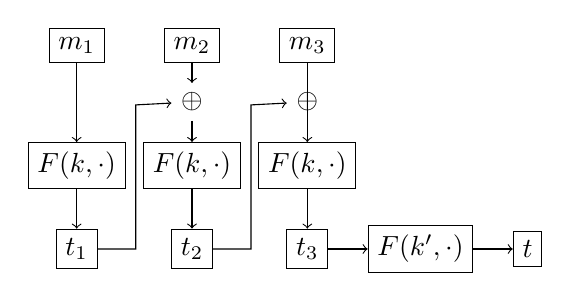
\begin{tikzpicture}
		\node (m0) [draw] {$m_1$};
    \node[below =1cm of m0] (f0) [draw] {$F(k, \cdot)$};
		\node[below =0.5cm of f0] (t0) [draw] {$t_1$};
		\draw [->] (m0) edge (f0) (f0) edge (t0);

		\node[right=0.75cm of m0] (m1) [draw] {$m_2$};
		\node[below =0.25cm of m1] (m1xt0) {$\oplus$};
		\draw [->] (t0) - ++(0.75,0) -- ++(0.75,1.83) -- (m1xt0);
    \node[below =1cm of m1] (f1) [draw] {$F(k, \cdot)$};
		\node[below =0.5cm of f1] (t1) [draw] {$t_2$};
		\draw [->] (m1) edge (m1xt0) (m1xt0) edge (f1) (f1) edge (t1);

		\node[right=0.75cm of m1] (m2) [draw] {$m_3$};
		\node[below =0.25cm of m2] (m2xt1) {$\oplus$};
		\draw [->] (t1) - ++(0.75,0) -- ++(0.75,1.83) -- (m2xt1);
    \node[below =1cm of m2] (f2) [draw] {$F(k, \cdot)$};
		\node[below =0.5cm of f2] (t2) [draw] {$t_3$};
    \node[right=0.5cm of t2] (out) [draw] {$F(k', \cdot)$};
    \node[right=0.5cm of out] (outp) [draw] {$t$};
		\draw [->] (m2) edge (f2) (f2) edge (t2);
    \draw [->] (t2) edge (out);
    \draw [->] (out) edge (outp);
	\end{tikzpicture}
  \caption{The CBC-MAC construction.}
	\label{fig:}
\end{figure}

CBC-MAC is going out of favor for two reasons:
\begin{enumerate}
  \item It is impossible to parallelize the MAC computation:
        the chaining procedure is inherently sequential so you 
        cannot speed it up, even if you have a computer with many 
        CPU cores.
  \item Computing the MAC requires one PRF invocation \emph{per block} of the message.
        There are even faster MACs that require only one PRF invocation
        \emph{per message} total, 
        plus a number of fast ``non-cryptographic'' operations
        per message block.
        These MACs can be faster than CBC-MAC on some processors.
        The GMAC construction we will see next is one example.
\end{enumerate}

% TODO: diagram

\subsection{A parallelizable MAC: Carter-Wegman MAC}\label{sec:mac:cw}

We now describe a different way to authenticate long messages.
This MAC scheme is parallelizable and also requires only one 
single PRF invocation per message authenticated (independent of
the message length).
The construction is named the Carter-Wegman MAC, after its
inventors.\cite{CW81}
Modern encryption schemes, including AES-GCM (\cref{sec:enc:gcm})
use a Carter-Wegman-style MAC as a key ingredient.

For this construction, we will use the notation
$\Z_p$ to indicate the set of integers modulo $p$
with addition and multiplication modulo $p$.
So $x + y \in \Z_p$ means that we add $x$ and $y$
as integers and reduce the result modulo~$p$.
Typically, we will think of $p$ as a prime---of
64 bits, for example.

The MAC uses a fixed a prime number $p$ as a parameter,
where $p \approx 2^n$ on security parameter $n$.\marginnote{So
in practice, we take $p \approx 2^{128}$
for 128-bit security.}
The MAC uses a pseudorandom function 
$F \colon \calK \times \Z_p \to \Z_p$.
\marginnote{Here, the input space of the pseudorandom 
function $F$ is the set of integers in $\{0, \dots, p-1\}$.
Given a pseudorandom function on bitstrings, it is indeed
possible to construct one that operates on numbers in 
$\Z_p$ like this by interpreting each number as a bitstring.}

The keyspace for the MAC is $\calK$, so the MAC key consists of a key for 
the pseudorandom function.
The message space for the MAC is $\calM = \Z_p^{\leq L}$,
the set of vectors of integers of $\Z_p$ elements of length
at most $L$ where $L \ll p$.
Here, assume that the message vector has length at least $1$.

One other difference is that this MAC construction is 
\emph{randomized}. So there are now two algorithms:
\begin{itemize}
  \item $\MACSign(k, m) \to t$, which takes as input a key $k$ and message $m$
        and outputs a MAC tag $t$, and 
  \item $\MACVerify(k, m, t) \to \zo$, which takes as input a key $k$,
    message $m$, tag $t$, and outputs an accept/reject bit.
\end{itemize}
The security definition here is essentially the same as for deterministic MACs,
except that we use different algorithms to generate and verify the MAC tags.

The Carter-Wegman MAC construction is then:

\medskip
\noindent
$\MACSign(k, m \in \Z^{\leq L}_p) \to t$.
\begin{itemize}[noitemsep]
  \item Compute $v \gets F(k, 0) \in \Z_p$.
  \item Parse the message into chunks as $(m_1, \dots, m_{\ell}) \gets m \in \Z_p^\ell$.
  \item Compute $M(v) \gets m_1 v + m_2 v^2 + m_3 v^3 \cdots + m_{\ell} v^{\ell} \in \Z_p$. \\
        \marginnote{Essentially we are viewing the blocks of the message 
        $m$ as coefficients of a degree-$t$
        polynomial $M(\cdot)$. We then evaluate this polynomial 
        at the secret point $v$ determined by the MAC key.}
        \hcg{Check the definition of the message polynomial $M$. Should 
        there be an additional $v^{t+1}$ monomial?}
  \item Sample a nonce $r \getsr \Z_p$.
  \item Output $t \gets \big(r, F(k, r) + M(v)\big) \in \Z^2_p$ as the MAC tag.
\end{itemize}

\medskip
\noindent
$\MACVerify(k, m, t) \to \zo$.
\begin{itemize}[noitemsep]
  \item Compute $v \gets F(k, 0) \in \Z_p$.
  \item Parse the message into chunks as $(m_1, \dots, m_{\ell}) \gets m \in \Z_p^\ell$.
  \item Compute $M(v) \gets m_1 v + m_2 v^2 + m_3 v^3 + \cdots + m_{\ell} v^{\ell}\in \Z_p$. \\
  \item Parse the tag $(r, z) \gets t \in \Z^2_p$.
  \item Output ``1'' if and only if $z - F(k, r) = M(v)$. 
\end{itemize}


\paragraph{Security intuition.}
\marginnote{For a detailed treatment of Carter-Wegman security 
see Boneh and Shoup's textbook, \emph{A Graduate Course in Applied Cryptography},
Section 7.4.}
The security argument here goes as follows:
\begin{itemize}
  \item First, we appeal to the PRF security property to argue
        that we can replace the values $F(k_F, r)$ used to generate
        the tags with truly random values.

  \item Next, we show that as long as the $\MACSign$ algorithm never
        samples the same nonce $r$ twice, the masking values $F(k,r)$
        are independent random values that complete hide the values $M(v)$.
        So, the adversary learns no information on the secret point $v$
        by making MAC queries.

  \item Now, say that the adversary finds a forged message-tag pair $(m^*, t^*)$.
    There are two cases:
        \begin{itemize}
          \item Either the forgery uses a fresh random nonce $r^*$ that did 
            not appear as the response to any of the adversary's MAC queries.
            In this case, the forgery is only valid with probability $1/p$. 
          \item Alternatively, the forger could use a random nonce $r^*$
            that is equal to the nonce $r$ returned from one of the adversary's
            MAC queries.
            In this case, we have the following relations, where message
            $m$ polynomial $M$ was the message the adversary queried of
            the challenger:
            \begin{align*}
              F(k, r) &= M(v) - z\\
              F(k, r) &= M^*(v) - z^*\\
              0 &= \big(M(v) - M^*(v)\big) + (z - z^*).
            \end{align*}
            Since $m \neq m^*$, we know $z \neq z^*$.
            So $(M(\cdot) - M^*(\cdot)) + (z^* - z)$ is a non-zero polynomial
            of degree at most $t$. 
            Since such a polynomial can have at most $\ell \leq L$ zeros in $\Z_p$,
            and since the adversaries view is independent of the evaluation
            point $v \in \Z_p$, the probability that the adversary's 
            forgery is valid is at most $\ell/p$.
        \end{itemize}

     In either case, the adversary's probability of forging is
     $O(L)/p = \poly(\lambda) \cdot \negl(\lambda) = \negl(\lambda)$
     on security parameter $\lambda$.
\end{itemize}




\chapter{Digital Signatures}

In the last section, our strategy for
authentication depended on two parties sharing a
secret key.
In that discussion, we completely left
out of the picture how these parties should
exchange this secret key.
Our implication was that they
went to some private room and exchanged the key in
secret, but in many cases this is not practical:
if they could whisper a key, why not just whisper the message?

Luckily, there is a way to get around this requirement for a shared secret using \emph{public-key cryptography}.\cite{DH76} % TODO: cite DH
\marginnote{The original Diffie-Hellman paper from 1976, which introduced
public-key cryptography, is a fascinating read.}

\section{Definitions}
The basic idea of public-key cryptography, applied
to authentication, is that each party will
generate two linked keys---a secret signing key
and a public verification key.
The verification key will be good enough to verify that a signature
is valid, but not to generate new signatures.

\begin{definition}[Signature Scheme]
	A signature scheme is associated with a message space $\calM$ and three efficient algorithms $(\Gen, \Sign, \Ver)$.

      \marginnote{In theoretical papers, people will write $\Gen(1^\lambda)$ to indicate that the key-generation
      algorithm takes as input a length-$\lambda$ string of ones.
      This is just a hack to make the input given to $\Gen$ $\lambda$ bits long so that the
      $\Gen$ algorithm can run in time polynomial in its input length: $\poly(\lambda)$.
      If we express $\lambda$ in binary, then $\Gen(\lambda)$ gets a $\log_2 \lambda$-bit input
      and can only run in time $\poly(\log \lambda)$.
      This distinction is really unimportant, but if you see the $1^\lambda$ notation, you will
      now know what it means.}
	\begin{itemize}
    \item $\Gen(\lambda) \to (\sk, \vk)$.
      The key-generation algorithm as input a security parameter $\lambda \in \N$ and outputs a secret signing key $\sk$ and public verification key $\vk$.
      The algorithm $\Gen$ runs in time $\poly(\lambda)$.
    \item $\Sign(\sk, m) \to \sigma$.
      The signing algorithm takes as input a secret key $\sk$ and a message $m \in \calM$, and outputs a signature $\sigma$.
    \item $\Ver(\vk, m, \sigma) \to \zo$.
      The signature-verification algorithm takes as input a public verification key $\vk$, a message $m \in \calM$, and a signature $\sig$, 
      and outputs $\bin$, indicating acceptance or rejection.
	\end{itemize}
	
\end{definition}

For a signature scheme to be useful, a correct verifier must always accept messages from an
honest signer. Formally, we have:

\begin{definition}[Digital signatures: Correctness]
  A digital-signature scheme $(\Gen, \Sign, \Ver)$ is \emph{correct} if,
  for all messages $m \in \calM$:
  \[ \Pr\big[\Ver(\vk, m, \Sign(\sk, m)) = 1 \colon (\sk, \vk) \gets \Gen(\lambda) \big] = 1. \]
\end{definition}

The standard security notion for digital signatures is very similar
to that for MACs (\cref{def:mac-sec}).
The only difference here is that a digital-signature scheme splits the single
secret MAC key into two keys: a secret signing key and a public verification key.
Otherwise the definition is essentially identical.

\begin{definition}[Digital signatures: Security -- existential unforgeability under chosen message attack]\label{def:sig-sec}
  A digital-signature scheme $(\Gen, \Sign, \Ver)$ is \emph{secure} if
  all efficient adversaries win the following security 
  game with only negligible probability:
  \begin{itemize}[noitemsep]
    \item The challenger runs $(\sk, \vk) \gets \Gen(\lambda)$ and sends $\vk$ to the adversary.
    \item For $i = 1, 2, \dots$  (polynomially many times)
      \begin{itemize}
        \item The adversary sends a message $m_i \in \calM$ to the challenger.
        \item The challenger replies with $\sigma_i \gets \Sign(\sk, m_i)$.
      \end{itemize}
    \item The adversary outputs a message-signature pair $(m^*, \sigma^*)$.
    \item The adversary wins if $\Ver(\vk, m^*, \sigma^*) = 1$ and $m^* \not \in \{m_1, m_2, \dots\}$.
  \end{itemize}
\end{definition}

Notice that the security definition here allows an attacker, given a valid
message-signature pair $(m, \sigma)$ to produce additional valid message-signature
pairs on the same message: $(m, \sigma'), (m, \sigma''), \dots$.
Standard digital-signature schemes, such as the elliptic-curve digital signature
algorithm (EC-DSA) have this property.

In some applications, we want to prohibit an attacker from finding \emph{any}
new message-signature pair. We call this security notion ``\emph{strong} existential unforgeability under chosen message attack.'' 

The definition is the same as in \cref{def:sig-sec} except that we require
the adversary to find a valid-message signature pair $(m^*, \sigma^*)$
such that $(m^*, \sigma^*) \not \in \{ (m_1, \sigma_1), (m_2, \sigma_2), \dots \}$.

\section{Constructing a Signature Scheme}
In the following sections, we will show how to construct a digital-signature
scheme from any one-way function (\cref{def:owf}).

We will generate a signature scheme that is secure, but that has a relatively large
signatures and public keys: to achieve security against attackers running
in time $2^\lambda$, this signature scheme has signatures of $O(\lambda^2)$ bits.
Widely used modern digital signature schemes (e.g., EC-DSA) have signatures
of $O(\lambda)$ bits.\marginnote{One benefit of the signature scheme that 
we present here is that---unlike EC-DSA, RSA, DSA, and other widely used
signature schemes---this one is plausibly secure even against \emph{quantum}
adversaries.\todo{Cite NIST PQ signature schemes and compare}
}

We will construct this scheme in three stages:

\begin{enumerate}
	\item Construct a \emph{one-time secure} signature scheme for \emph{fixed-length messages}.
        With this scheme, an attacker who sees two signatures under the same signing key can forge signatures.
        In addition, the secret signing key for this scheme will be larger than the size of the message 
        being signed.
      \item Construct a \emph{one-time secure} scheme for \emph{arbitrary-length messages}.
        Here, we construct a one-time signature scheme whose secret signing key is independent of 
        the length of the signed message.

      \item Construct a \emph{many-time secure} scheme (i.e., a fully secure one under 
        \cref{def:sig-sec}) for \emph{arbitrary-length messages}.
        This last scheme is a fully secure and fully functional digital-signature scheme.
\end{enumerate}


\section{One-time-secure Signatures (Lamport Signatures)}

In this section we give a very simple and elegant construction 
of one-time-secure digital signatures, due to Lamport.\cite{L79}
Before giving the construction, we define one-time security for 
digital-signature schemes.
This signature scheme is not generally useful on its own, but is
useful as a building block.

\begin{definition}[Digital signatures: One-Time Security]\label{def:sig-once}
A digital-signature scheme $(\Gen, \Sign, \Ver)$ over message space $\calM$ is \emph{one-time secure} if all efficient adversaries win
the following game with negligible probability:
  \begin{itemize}[noitemsep]
    \item The challenger generates $(\sk, \vk) \leftarrow \Gen(\lambda)$ and sends $\vk$ to the adversary.
    \item The adversary sends the challenger \emph{single} message $m \in \calM$.
    \item The challenger responds with $\sig = \Sign(\sk, m)$.
    \item The adversary outputs $(m^*, \sig^*)$.
    \item The adversary wins the game if $\Ver(\vk, m^*, \sig^*) = 1$ and $m^* \neq m$.
\end{itemize}
\end{definition}

\paragraph{Lamport signatures.}
We now construct a one-time secure signature scheme for messages in $\bin^n$,
for some fixed message length $n \in \N$. 
To do this, we will define the following algorithms, which make use of a
one-way function $f \colon \calX \to \calY$:
\begin{itemize}
  \item $\Gen() \to (\sk, \vk)$. 
    \marginnote{In this construction, we leave the security parameter $\lambda$
    implicit.
    To be fully formal, $\Gen$ would take $\lambda$ an input.
    The one-way function $f$ and its domain $\calX$ would both
    depend on $\lambda$. So we would write $f_\lambda$ and $\calX_\lambda$.
    }
    Choose $2n$ random elements from $\calX$,
    the domain of the one-way function $f$.
    Arrange these values in to a $2 \times n$
    matrix, which forms the secret signing key $\sk$.
    The public verification key just consists of the $2n$
    images of these values under the one-way function $f$:
\[ \sk \gets \begin{pmatrix}
	x_{10} & \ldots & x_{n0} \\
	x_{11} & \ldots & x_{n1} \\
	\end{pmatrix},\quad \vk \gets \begin{pmatrix}
	f(x_{10}) & \ldots & f(x_{n0}) \\
	f(x_{11}) & \ldots & f(x_{n1}) \\
\end{pmatrix}.\]
	\item $\Sign(\sk, m) \to \sigma$ outputs $(x_{1m_1}, \ldots x_{nm_n})$, where $m_1 \dots m_n$ 
    are the individual bits of the length-$n$ message $m \in \zo^n$.
	\item $\Ver(\vk, m, \sig) \to \zo$ parses the 
    the message into bits $m = m_1\dots m_n \in \zon$ and
    the signature $\sig$ into its individual symbols $\sig = (x_1^*, \ldots x_n^*) \in \calX^n$.
    The signing routine accepts if, for all $i \in \{1, \dots, n\}$:
    \begin{equation}
      f(x^*_i) = \vk_{i,m_i}.\label{eq:lamport}
    \end{equation}
    In other words, the routine accepts if applying the one-way function $f$ to each symbol
    of the signature matches the corresponding value in the verification key.
    (Otherwise, the signing routine rejects.)
\end{itemize}

This signature scheme has relatively large keys:
the verification key, in particular consists of $2n$ values,
where each is of length $\Omega(\lambda)$ bits.
So the total length is roughly $2n\lambda$ bits---much
longer than the $n$-bit message being signed.

In addition, notice that an adversary who sees signatures
on even two messages can forge signatures on messages of its choice.
In particular:
\begin{itemize}[noitemsep]
  \item The adversary first asks for a signature on the message $m_0 = 0^n$.
It receives $\sig_0 = (x_{10}, \ldots, x_{n0})$.
  \item The adversary then then asks for a signature on the message $m_1 = 1^n$.
    It receives $\sig_1 = (x_{11}, \ldots, x_{n1})$.
  \item At this point, the adversary has the entire secret signing key! 
\end{itemize}
However, we will show that this scheme is indeed one-time secure.

\begin{claim} 
The Lamport signature scheme is one-time secure under the
assumption that $f$ is a one-way function.
\end{claim}
\marginnote{Remember that if $\classP = \classNP$, 
one-way functions, and also digital signature schemes, do not exist. 
So any proof of security of a digital-signature scheme will require
some sort of cryptographic assumption.}

In cryptography, we generally prove these security
claims by \emph{reduction}: we will show that
if there exists an efficient adversary $\calA$
that breaks the security of our scheme,
then we can construct an efficient adversary $\calB$ 
that breaks one of our assumptions.
If we do this, we have reached a contradiction to one
of our assumptions, so the first adversary cannot exist.

\begin{proof}[Proof of Claim]
Suppose there exists an adversary $\A$ that wins the 
one-time-security game of \cref{def:sig-once} with non-negligible probability $\epsilon$.
That is, the adversary can produces $(m^*, \sig^*)$ such that $\Ver(\vk, m^*, \sig^*) = 1$ and $m \neq m^*$ given only $\sig = \Sign(\sk, m)$.
We can then construct an adversary $\B$ that can use $\A$ to 
invert the one-way function.

\marginnote{Lamport's construction shows that if one-way functions
exist, then so do digital signatures.
Can you show that if digital signatures exist, then so do one-way
functions?}

In particular, our adversary $\calB$ will use algorithm $\calA$
as a subroutine to invert the one-way function.
We will show that if $\calA$ wins in the one-time signature security
game often, then algorithm $\calB$ will invert the one-way function
often, which is a contradiction.

Assume our one-way function is of the form $f \colon \calX \to \calY$
and that the Lamport signature scheme is on $n$-bit messages.
The one-way-function adversary $\calB$ operates as follows:
\begin{itemize}[noitemsep]
  \item The adversary $\calB$ is given a point $y \in \calY$
    and its task is to produce a preimage of $y$ under $f$. 
  \item The adversary $\calB$ generates a signing keypair as follows:
    \begin{itemize}[noitemsep]
      \item It runs the key-generation algorithm for the Lamport signature scheme $(\sk, \vk) \gets \Gen()$.
      \item The adversary chooses a random value $i^* \getsr \{1, \dots, n\}$
            and a random bit $\beta^* \getsr \zo$.
          \item The adversary sets $\vk_{i^*,\beta^*} \gets y$.
            That is, it inserts the one-way-function point it must invert
            into a random location in the verification key.
    \end{itemize}
  \item The adversary then sends the verification key $\vk$ to the Lamport-signature adversary $\calA$.
  \item The adversary $\calA$ asks for the signature on a message $m = m_1 m_2 \dots m_n \in \zon$.
  \item If $m_{i^*} = \beta^*$, then algorithm $\calB$ cannot produce a valid signature on the message
        $m$ and it outputs FAIL.
  \item Otherwise, the algorithm $\calB$ returns the signature $\sigma = (\sk_{1,m_1}, \dots, \sk_{n,m_n}) \in \calX^n$
        to algorithm $\calA$.
  \item Algorithm $\calA$ then produces a forged message-signature pair $(m^*, \sigma^*)$,
        where $m \neq m^*$.
  \item Algorithm $\calB$ parses $m^* = m^*_1 \dots m^*_n \in \zon$
        and $\sigma^* = \sigma^*_1 \dots \sigma^*_n \in \calX^n$. Then:
        \begin{itemize}[noitemsep]
          \item If $m_{i^*} = m_i$, algorithm $\calB$ outputs FAIL.
          \item Otherwise, algorithm $\calB$ outputs $x \gets \sigma^*_{i^*} \in \calX$.
        \end{itemize}
\end{itemize}

First, notice that whenever $(m^*, \sigma^*)$ is a valid message-signature
pair and whenever algorithm $\calB$ does not output FAIL, algorithm $\calB$
outputs a preimage $x \in \calX$ of point $y \in \calY$ under the one-way function $f$.
That is because, by the verification relation (\ref{eq:lamport}) for Lamport signatures,
\[f(x) = f(\sigma^*_{i^*}) = \vk_{i^*,m^*_{i^*}} = \vk_{i^*, 1 - m_i} = \vk_{i^*, \beta^*} = y.\]

Now, we must show that algorithm $\calB$ does not output FAIL too often.
Since algorithm $\calB$ chooses the values $i^*$ and $\beta^*$ at random,
and since the adversary $\calA$ behavior is \emph{independent} of these values,
we can say:
  \begin{itemize}
    \item the probability of the first failure event is $1/2$,
          since there are two possible choices of $m_{i^*}$ and only 
          one of these is bad, and 
    \item the probability of the second failure event is at most $1/n$,
          since $m$ and $m^*$ must differ in at least one of $n$ bits,
          and there is a $1/n$ probability that this differing bit is
          at index $i^*$.
  \end{itemize}

The events that $\calA$ breaks the signature scheme
and that either of these failures occur are all \emph{independent}.
Then if $\calA$ breaks the one-way function with probability $\epsilon$,
our one-way-function adversary $\calB$
inverts the one-way function with probability
\[ \epsilon_\text{one-way} = \epsilon \cdot \frac{1}{2} \cdot \frac{1}{n}.\]

The probability of either bad is at most $1/2 + 1/n$,
by the union bound.
Therefore if algorithm $\calA$ breaks one-time security of Lamport's
scheme with probability $\epsilon$,
If $\epsilon$ is non-negligible, then $\epsilon_\text{one-way} = \epsilon/2n$
is also non-negligible, and we have a contradiction.
\end{proof}


\backmatter

%%% BIBLIOGRAPHY
%%% -------------------------------------------------------------
\bibliographystyle{plain}
\bibliography{ref}


\end{document}
